\documentclass[11pt]{article} % Adding 'twocolumn' for two-column layout
\usepackage[margin=0.75in]{geometry} % Setting custom margins
\usepackage{amsmath}
\usepackage{graphicx}
\usepackage{subcaption} % Add this package in your preamble if not already included
\usepackage{placeins} 

\usepackage{multicol}
\usepackage{float}

\usepackage[numbers]{natbib} % Enabling numeric citations with natbib

\usepackage{pdflscape} %for bigger tables and figures allows to input a landscape page

\usepackage{array} %to fit the text on tables without justify
\usepackage{url}
\usepackage[toc,page]{appendix} % For appendix support


\title{Comparative Efficacy of PET/CT and PET/MR in Precision Radiotherapy for Liver Cancer: Advances in Dosimetry and Tumor Delineation}
\author{Daniel Juarez}
\date{\today}

\begin{document}

\maketitle

\begin{multicols}{2}

% ============================
% Include Sections
% ============================

\section{Introduction}
% ============================
% Section: Introduction
% ============================

%\subsection{The Role of Imaging in Radiation Therapy}

During all stages of radiotherapy, getting the sense of where health professionals focus their work and the methods used to shape or conform the target tissue is of most vital importance. This information is provided by different imaging devices and techniques molded to each different case. During planning, images help visualize target lesions and clarify which pathway and devices are best to use. This information serves as a guide to determine patient and device position. During treatment, it provides insight into treatment outcomes and potential complications \cite{decazes2021}. Finally, during surveillance or control, it gives the comparison point to check accuracy and success while pointing to the right direction to follow.

The preferred imaging modality for all types of cancer diagnosis is Computed Tomography (CT), this is due to it high-resolution anatomical detail and the information provided to map tissue electron density \cite{decazes2021,yan2024}. However, like every imaging modality, CT has its limitations, emphazising the need for complementary imaging techniques, especially for precise tumor targeting in complex cases like liver cancer \cite{yan2024}.

%\subsection{Hybrid Imaging for Enhanced Accuracy}
For these reason, no single imaging modality is entirely sufficient for an absolute precise role in radiation therapy due to intrinsic trade-offs \cite{decazes2021}.Setting CT aside, another good alternative is Magnetic Resonance Imaging (MRI), although valuable for soft tissue delineation, it lacks electron density information, making them less suitable as a standalone modalities in radiotherapy \cite{decazes2021}. Another alternative is Positron Emission Tomography (PET), which provides a new lens since it contributes with unique metabolic information that complements anatomical imaging and aids in tumor delineation \cite{decazes2021}.

Exploring new techniques, technologies and pathways of using existing devices are carefully studied. Hybrid techniques are of most interest such as PET/CT and PET/MR. These modalities aim to overcome limitations by combining the strengths of each modality.

The objective of this paper is to compare PET/CT and PET/MR in liver cancer radiotherapy, focusing on their applications in tumor delineation and dosimetric planning, and patient monitoring. An evaluation of their technical capabilities, clinical integration, and implications for adaptive radiotherapy workflows will be inlcuded. The aim is to explore how these hybrid modalities can enhance precision in liver cancer management. 

Table \ref{tab:modality_comparison} provides a comparative overview of the relevant used imaging modalities in radiotherapy, it includes technical complexity and workflow integration that may be overlooked. Each modality has specific roles, because of it no single technique is entirely sufficient for precise tumor targeting. Following the table an explanation of each modality and why hybrid approaches are needed is explained.

\end{multicols}
%merge Decazes and Yan
%Decazes TABLE 1 | Comparison of PET/MRI and other conventional image-based modalities in radiotherapy
%Yans TABLE 1 | Summary of advantages and disadvantages of CT, MRI, and PET separately and combined in PET/CT/MRI
%Yans TABLE 3 | Comparison of different imaging methods (star ranking)

\begin{landscape}
\begin{table}[H]
	\centering
	\renewcommand{\arraystretch}{1.5} % Adjust the multiplier (e.g., 1.5 for 50% more spacing)
	\setlength{\tabcolsep}{6pt} % Optional: Adjust column padding if needed
	\begin{tabular}{|l|>{\raggedright\arraybackslash}p{3.5cm}|>{\raggedright\arraybackslash}p{2.3cm}|>{\raggedright\arraybackslash}p{5.5cm}|>{\raggedright\arraybackslash}p{4.5cm}|>{\raggedright\arraybackslash}p{4.5cm}|}
		\hline
		\textbf{Modality} & \textbf{Diagnostic Information} & \textbf{Soft Tissue Resolution} & \textbf{Radiation Dose} & \textbf{Technical Complexity} & \textbf{Workflow Integration} \\ \hline
		CT & Anatomy and tissue electron density & Moderate (1 mm spatial resolution) & Ionizing radiation (higher dose) & Widely available; simple infrastructure requirements & Integrates easily into standard radiotherapy workflows; rapid acquisition \\ \hline
		MRI & Anatomy and function & Excellent (soft tissue contrast) & None (non-ionizing) & Requires trained personnel; specialized infrastructure & Long scan times; challenges with integration into dose planning workflows \\ \hline
		PET & Metabolic and functional imaging & Poor (blurred edges, partial volume effects) & Ionizing radiation (tracer-based) & Limited isotope availability; moderate complexity   & Requires co-registration with CT or MRI; \\ \hline
		PET/CT & Combines anatomical and functional imaging; provides BTV and GTV delineation & Moderate & Higher due to combined CT dose & Standardized; relatively simple calibration & Commonly used in clinical settings \\ \hline
		PET/MRI & Combines superior soft tissue contrast with metabolic imaging; pseudo-CT for dose calculation & Excellent & Reduced radiation compared to PET/CT & High complexity; limited infrastructure and operator expertise & Workflow integration less standardized compared to PET/CT \\ \hline
	\end{tabular}
	\caption{Comparison of imaging modalities (CT, MRI, PET, PET/CT, and PET/MRI) for radiotherapy applications. Adapted from Decazes et al. \cite{decazes2021}, Yan et al. \cite{yan2024}, and Knešaurek et al. \cite{knesaurek2018}.}
	\label{tab:modality_comparison}
\end{table}
\end{landscape}

\begin{multicols}{2}

First, CT is the standard modality used in radiotherapy due to its high anatomical resolution and integration into treatment workflows. However, it relies on ionizing radiation and it has moderate soft tissue resolution that limits its standalone use in complex cases, such as tumors adjacent to sensitive soft tissues. 

Next, MRI provides a solution to CT soft tissue resolution and adds functional imaging without ionizing radiation, making it ideal for delineating tumors in challenging areas.  Nevertheless, its known for long scan times and the difficulty to integrate electron density information of the tissue on the treatment plan. 

Then, PET offers a unique insight on tumor activity, that is functional and metabolic imaging. Still, its limitations are quite considerable, mainly poor spatial resolution which makes this modality rely on co-registration with anatomical modalities like CT or MRI. 

Following that, PET/CT solves these limitations by combining the anatomical clarity of CT with the functional insights of PET. Yet, the combined radiation dose remains a concern. 

Finally, PET/MRI merges superior soft tissue delineation with metabolic imaging. This modality reduces radiation exposure compared to PET/CT but faces significant challenges in technical complexity, cost, and workflow integration.

Imaging modalieties are complementary in nature because there are trade offs and risks on each of them. While CT and MRI is great in anatomical and soft tissue imaging, respectively, and PET provides metabolic insights, their integration through hybrid systems like PET/CT and PET/MRI is essential for achieving optimal precision in radiotherapy.\cite{decazes2021, yan2024}. Table \ref{tab:modality_comparison} convey the importance of advancement in hybird techniques to overcome the limitations of individual modalities and confidentely approach any complex clincal scenarios with either IMRT or VMAT as treatment.



\section{Background}
% ============================
% Section: Background
% ============================

% General background information about liver cancer and imaging.
%liver cancer types

%\subsection{Liver Cancer Overview}
%\subsection{PET/CT vs. PET/MR in Liver Cancer Radiotherapy}
Liver cancer is particularly difficult to diagnose and its treatment requires highly precise imaging. It needs accurate tumor delineation and because of its size and location spare healthy liver tissue, and organs at risk (OAR). This means radiologists need accuracy, especially when administering targeted therapies \cite{beaton2019, floridi2022}.

Around the world there is a common concern of cancer incidences. Liver cancer, in particular, ranks as the sixth most common diagnosed cancer and the third leading cause of cancer-related deaths. In 2020, approximately 905,700 new cases and 830,200 deaths were reported globally \cite{journal_of_hepatology2022}. 


The global burden varies significantly by region, for example, East Asia and sub-Saharan Africa have the largest incidence rate while in the United States liver cancer rates are comparatively lower. Global predictions estimate that this rates will increase by 55\% between 2020 and 2040, potentially leading to 1.4 million new cases and 1.3 million deaths annually by 2040 \cite{journal_of_hepatology2022}.

The American Cancer society projected approximately 41,630 new cases and 29,840 deaths in the United States \cite{cancer_stats2024}. As the year concludes we may expect to see the actual increase in new cases, however there is a historical increasing trend, the United States have seen, between 1975 and 2017, an increase of 228\% incidence and 137\% rise in mortality. Probably driven by a combination of rising risk factors, aging populations, and improved detection. However, despite advancements in imaging and treatment, late diagnoses and limited therapeutic options have contributed to persistently high mortality rates.

Moreover, projections made in 2020 suggest that liver cancer could become the third leading cause of cancer-related deaths in the US by 2030, surpassing breast, prostate, and colorectal cancers \cite{aacr_2030}. This is particularly interesting, since this has already happen globally, the slower growth of cases an mortality in the U.S. suggests that public health efforts are having a meaningful impact, continued advancements in imaging, personalized therapy, and public health interventions are needed to sustain and further improve outcomes.

%\subsection{Why is Liver Cancer Hard to Diagnose?}
The liver is the largest solid organ located in the upper right quadrant of the abdominal cavity, beneath the diaphragm, its roles includes metabolism, detoxification, and digestion. It is partially shielded by the rib cage, making it relatively protected. To better illustrate its position and function figure \ref{fig:liver-relations} shows the abdominal cavity with the liver’s relationship to adjacent organs such as the stomach, diaphragm, and intestines \cite{lecturio2023,ozmen2020}. 

\begin{figure}[H] % H ensures the image is placed exactly here (requires float package)
	\centering
	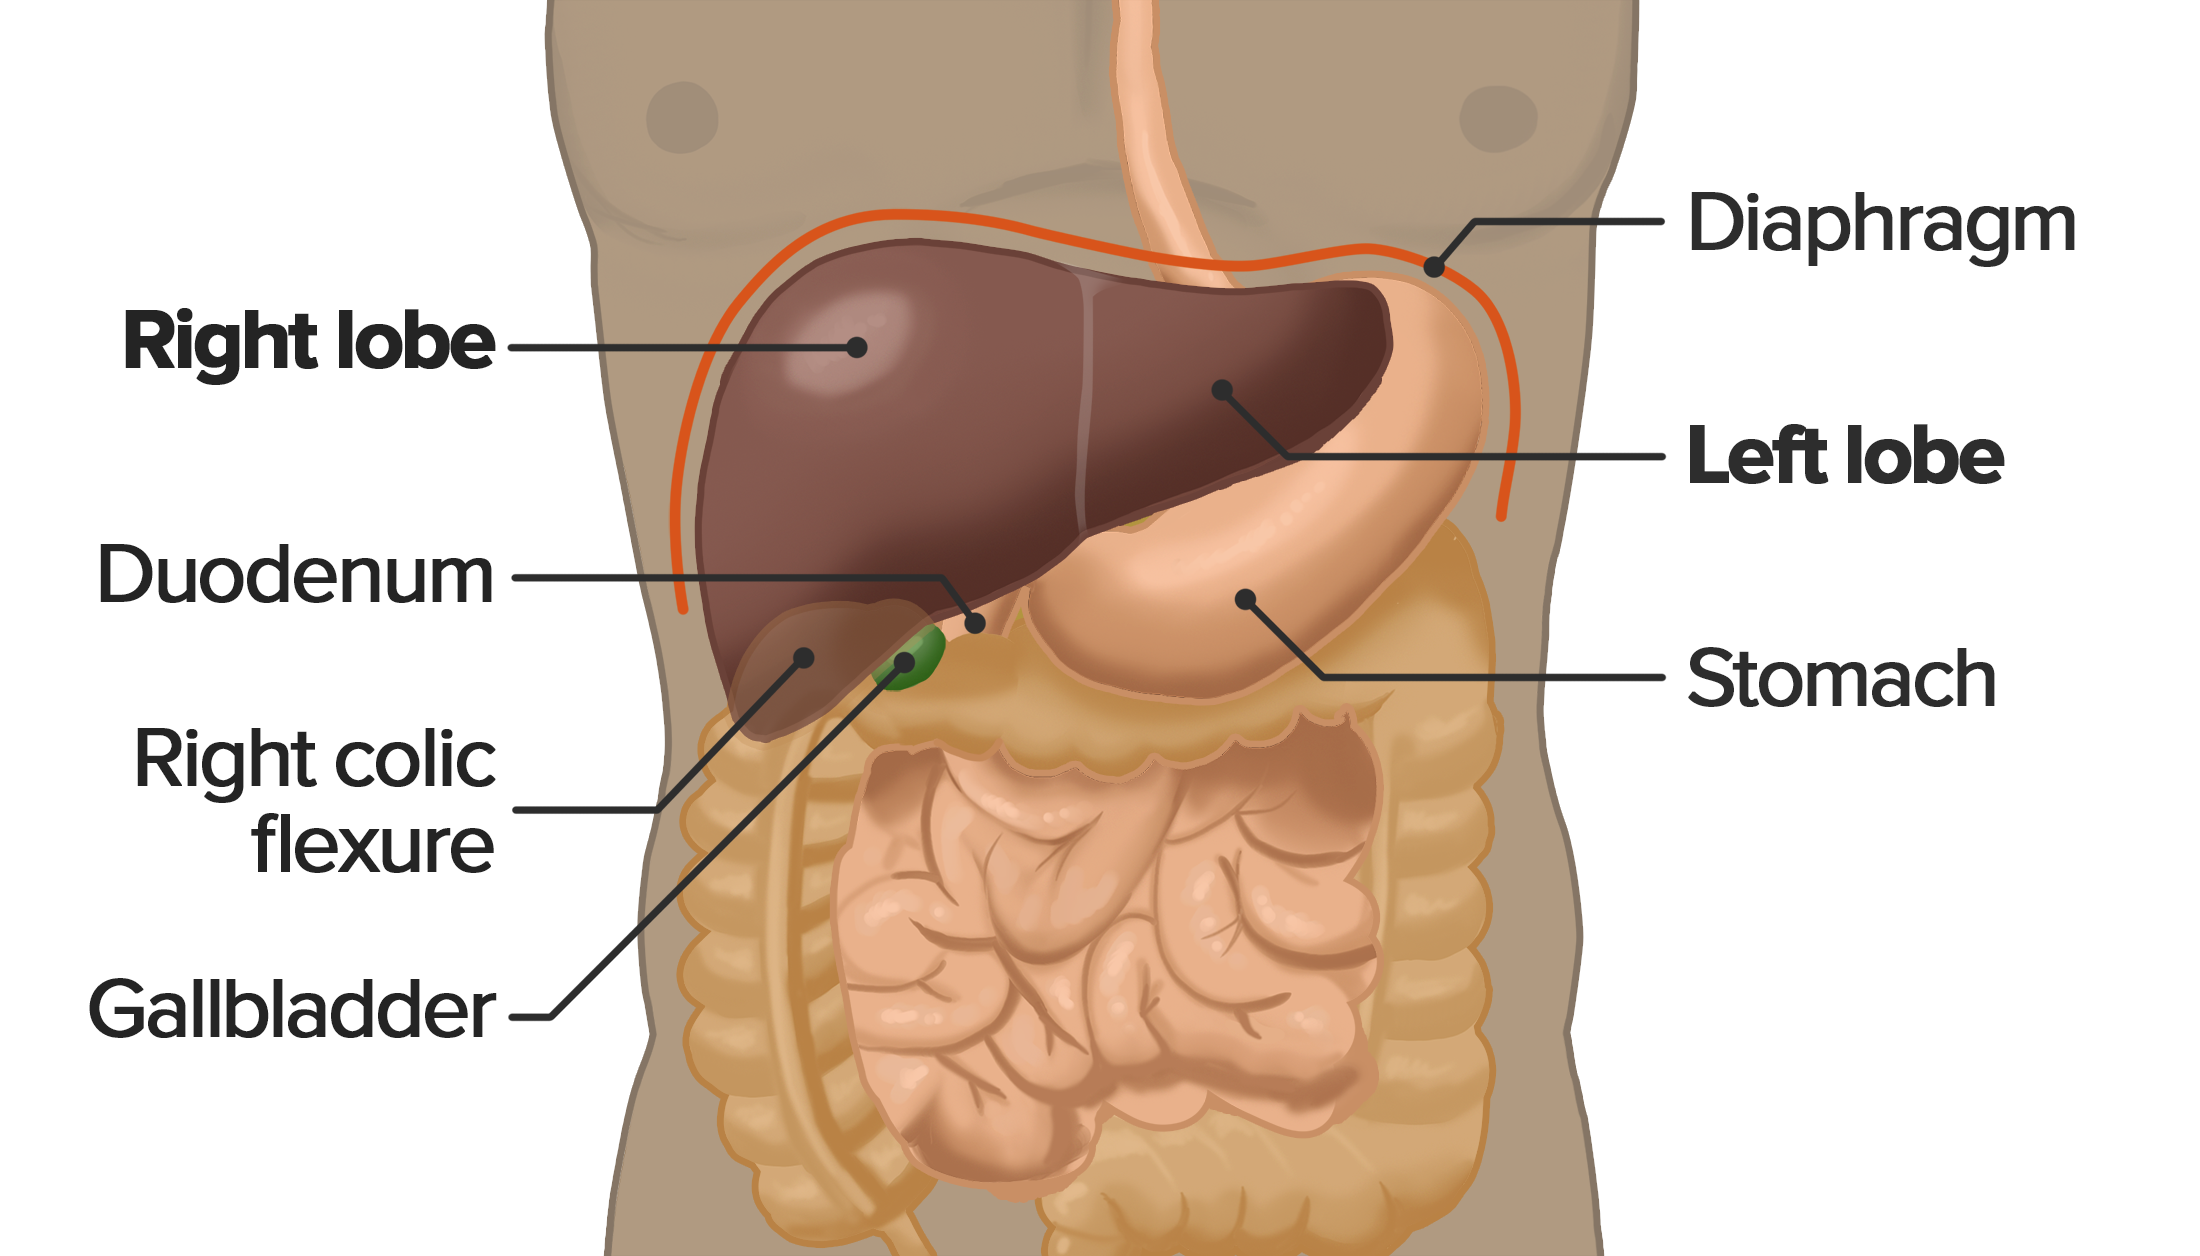
\includegraphics[width=0.5\textwidth]{assets/Liver-relations.png} % Adjust width as needed
	\caption{Anatomical Relations of the Liver}
	\label{fig:liver-relations}
\end{figure}

It has a complex structure, it has two main lobes (right and left), the right lobe is significantly larger, and its main function is metabolic and detoxification processes. The left lobe, is smaller, and it is in charge of production and nutrient metabolism \cite{ozmen2020}.

The liver can be shaped differently between individuals. As shown in Figure \ref{fig:liver-shapes}, the anterior surface of the liver can be classified into four primary shapes.

First, \textbf{Globular Shape (A)} A rounded configuration typically seen in healthy individuals with an average body. Next, \textbf{Conical Shape (B)} Characterized by a narrow right lobe and a smaller left lobe, often observed in elongated torsos. Then, \textbf{Quadrilateral Shape (C)} Exhibits a broader and flatter right lobe with minimal reduction, common in individuals with higher abdominal fat deposition. Finally, \textbf{Rectangular Shape (D)} A flat and wide configuration with a reduced height-to-width ratio \cite{ozmen2020,diagnostics13142371}.


\begin{figure}[ht]
	\centering
	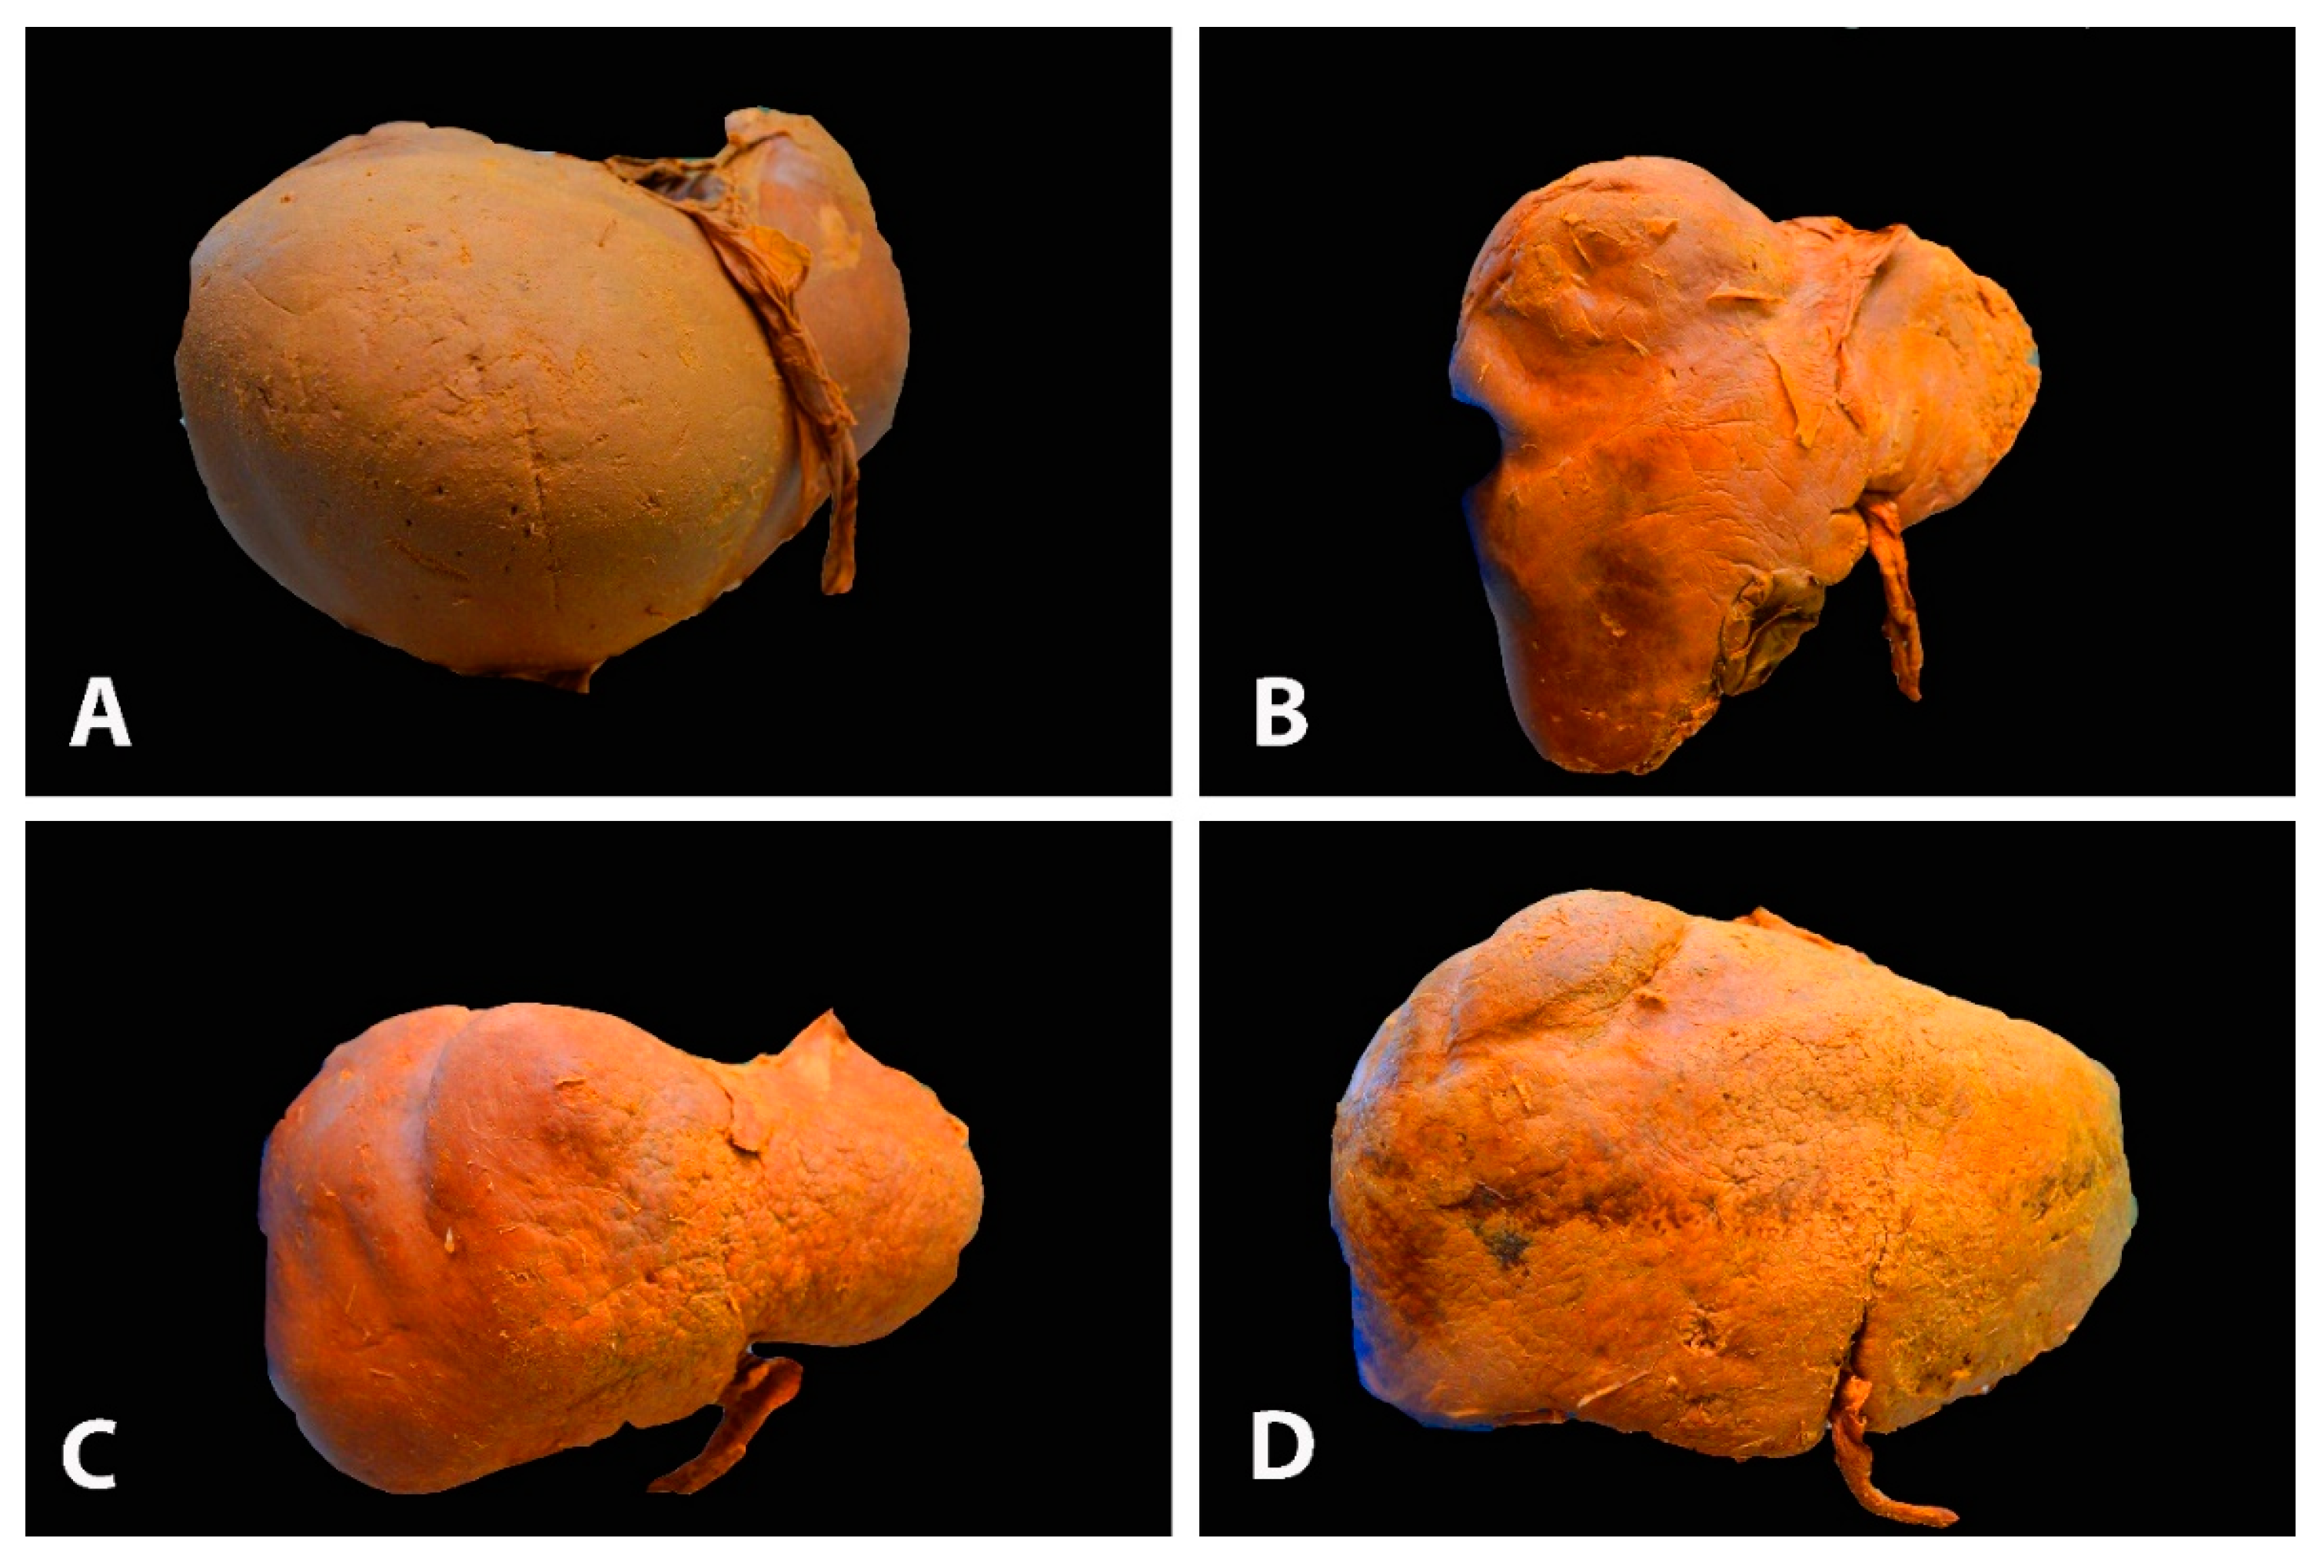
\includegraphics[width=0.45\textwidth]{assets/diagnostics-13-02371-g001.png} % Adjust path to include the relevant figure
	\caption{Anterior surface of the liver classified into four primary shapes: (A) Globular, (B) Conical, (C) Quadrilateral, and (D) Rectangular.}
	\label{fig:liver-shapes}
\end{figure}

Morphological variations directly impact diagnostic accuracy, treatment planning, and therapeutic outcomes. Changes in liver shape due to conditions such as cirrhosis or hepatic steatosis further complicate the diagnostic process, as these conditions alter the liver’s texture and vascular patterns. This can make it challenging to distinguish between benign and malignant lesions on imaging modalities like CT or MRI. Then, the liver is divided into eight segments by functionally, each segment is independent, receiving its own blood supply from a branch of the hepatic artery and portal vein and draining bile through a corresponding biliary branch. This segmention allows precision on diagnostics, surgery and transportation and is depicted on figure \ref{fig:liver-segments-side-by-side} \cite{diagnostics13142371}.

\begin{figure}[H]
	\centering
	\begin{subfigure}[t]{0.25\textwidth}
		\centering
		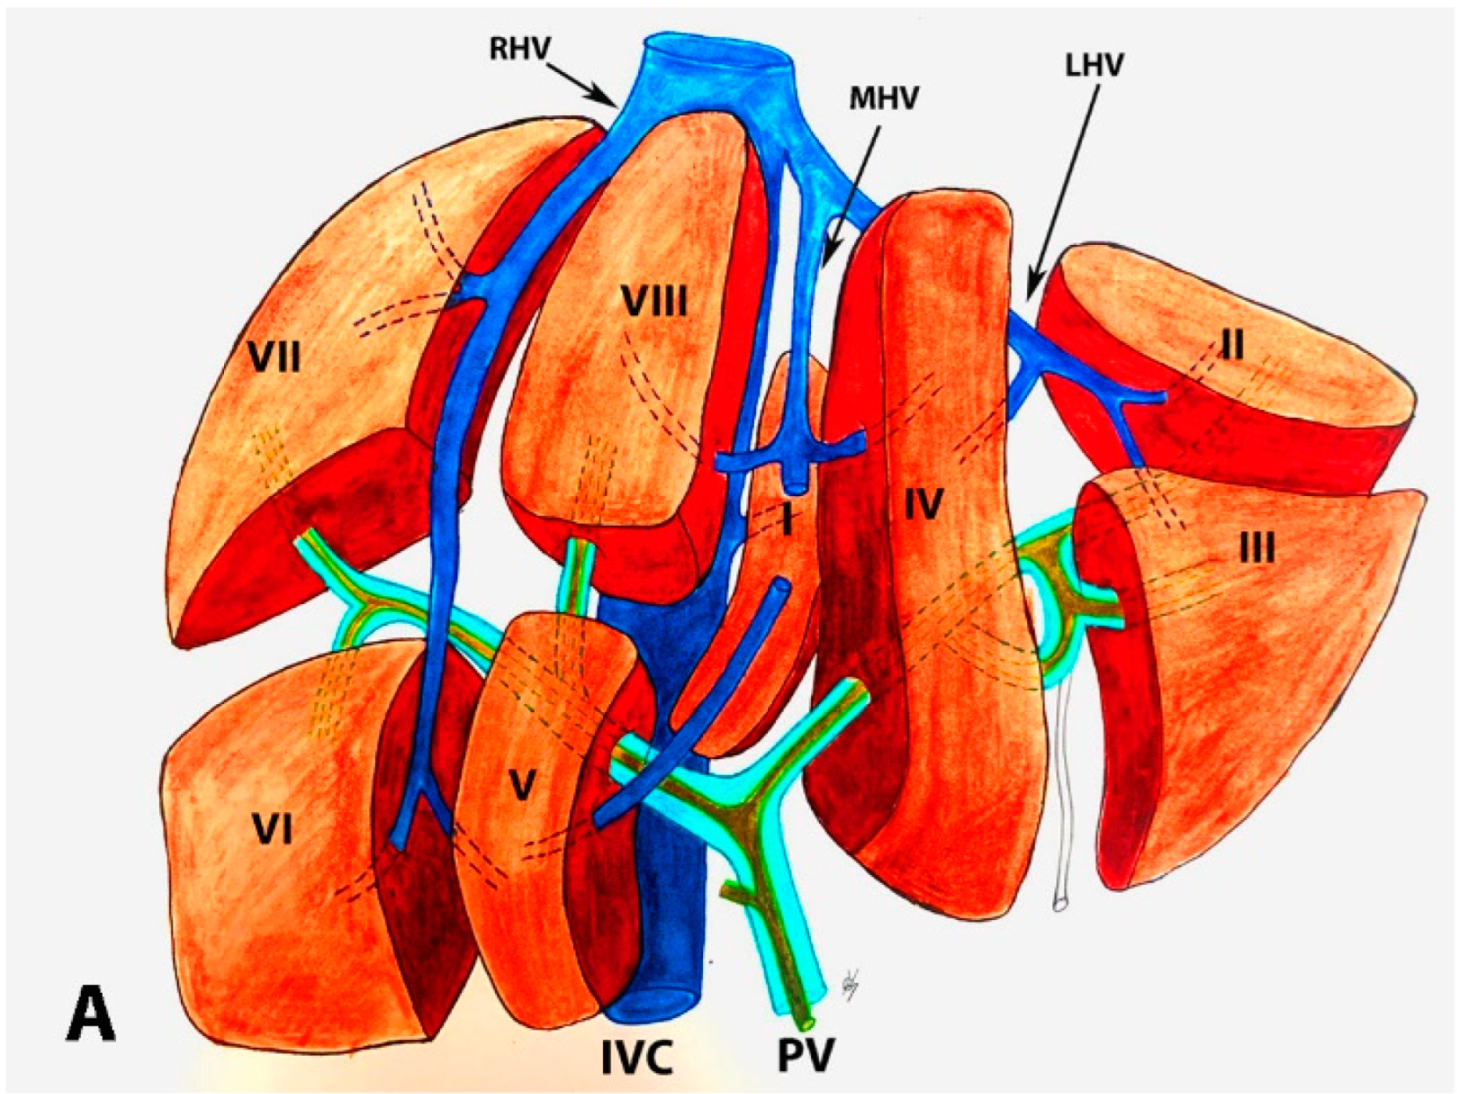
\includegraphics[width=\textwidth]{assets/figure_a.png} % Adjust path if needed
		\caption{}
		\label{fig:figure-a}
	\end{subfigure}
	\hfill
	\begin{subfigure}[t]{0.25\textwidth}
		\centering
		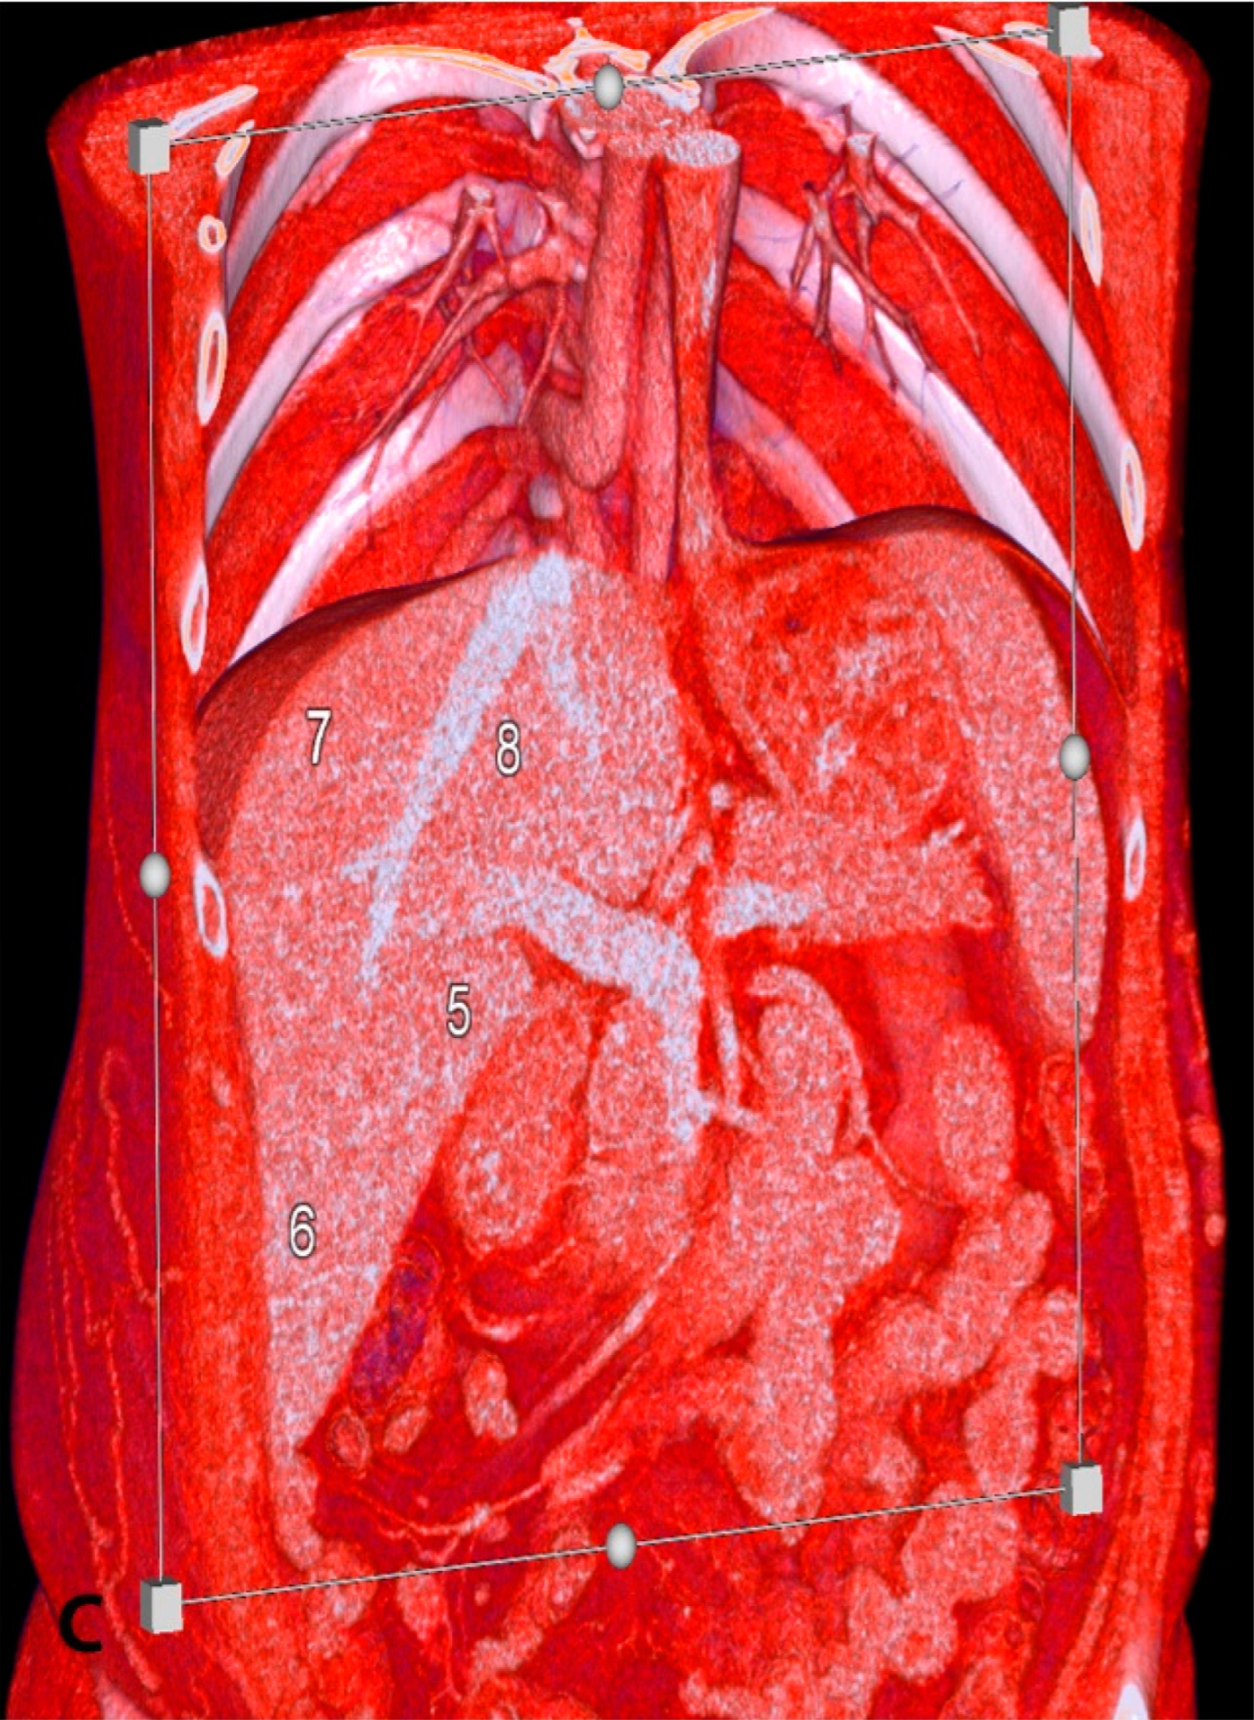
\includegraphics[width=\textwidth]{assets/figure_c.png} % Adjust path if needed
		\caption{}
		\label{fig:figure-c}
	\end{subfigure}
	\caption{Segments of the liver according to Couinaud’s classification: (A) ex vivo appearance; (C) coronal volume-rendered abdominal CT image with annotated right hepatic lobe segments. PV – portal vein; IVC – inferior vena cava.}
	\label{fig:liver-segments-side-by-side}
\end{figure}

The segmented and lobular structure of the liver makes imaging harder. Lesions can be difficult to localize within segments because of overlapping vascular and biliary structures. Small tumors or anomalie in deeper segments like the caudate lobe, which is encircled by other liver regions and  organs, may not be detected. \cite{WJGnet2023,liverMassCharacterization2023}

In radiotherapy, the morphological irregularities, may shift the relative position of tumors within the liver. This necessitates advanced imaging techniques, to precisely map the tumor’s location relative to moving anatomical structures like the diaphragm during the breathing cycle. \cite{luersen2015}

Moreover, the liver’s segmented anatomy and its dual blood supply necessitate careful dosimetric planning to optimize radiotherapy. Variations in lobe size affect the volume of liver tissue exposed to radiation. Additionally, exaggerated organ motion during respiration require adaptive radiotherapy techniques, such as respiratory gating or motion management systems, to ensure accurate dose delivery.\cite{pmc5658876}

Dosimetric planning techniques, such as Intensity-Modulated Radiation Therapy (IMRT) and Volumetric Modulated Arc Therapy (VMAT), take these variations into account by adapting dose distribution to the unique anatomy of each patient, sparing healthy tissues and minimizing complications. \cite{oymak2022}

Diagnosing cancer is a challenge also due to its nature, in particular liver cancer as it presents asymptomatic in early stages, for example hepatocellular carcinoma (HCC) often develops in patients with chronic liver disease or cirrhosis, which can mask early signs of cancer and further complicate detection \cite{quaglia2018,doi:10.1148/radiol.14132362}.

In the other hand there is limitations of standard screening tools, following the HCC example, usually tested with ultrasound and often combined with alpha-fetoprotein (AFP) test. AFP is a serum biomarker commonly used in HCC screening and diagnosis. AFP level increased may suggest underlying pathology, which may be malignant \cite{bialecki2005}.
However, ultrasound and AFP tests have limitations. Ultrasound sensitivity is hindered particularly in patients with obesity or cirrhosis.\cite{floridi2022} Studies have shown that ultrasound can miss more than half of early-stage tumors, while the addition of AFP testing still fails to detect over one-third of early HCC cases \cite{mcmahon2023}.

%\subsubsection{Challenges and Advances in Imaging for Liver Cancer}

Recent years have seen advancements in imaging techniques by combining standard techniques such as CT, MRI, and cone-beam CT (CBCT) to enhance tumor visualization.\cite{floridi2022}.

Imaging the liver is quite difficult due to its location beneath the rib cage, the impact of respiratory motion, and patient-specific factors or comorbilities. The liver’s heterogeneity and its internal complexity further complicate image interpretation. \cite{ferraioli2018}.

Imaging is useful during all stages of treatment. Because of the liver's intricate structure and common comorbidities such cirrhosis, it is important to accurately define tumor borders, determine vascular involvement, and estimate closeness to other tissues \cite{floridi2022}.

The most widely used imaging modality to asses liver cancer is ultrasound (US) due to its accessibility, real-time imaging capability, ability to assess blood flow via Doppler techniques, and because of its non-ionizing nature. But, it is limited by operator skill and sensitivity while detecting small lesions, in early-stage hepatocellular carcinoma (HCC) the smallest detectable lesions typically range from 3 to 5 mm in diameter. \cite{mcmahon2023,ferraioli2018}. 

For instance, small hepatic adenomas, which are benign solid lesions, often remain undetected until they grow larger than 5 cm. Similarly, early-stage intrahepatic cholangiocarcinoma, a bile duct cancer, and small hepatic cysts, which are fluid-filled sacs, are frequently missed unless they become symptomatic or increase in size \cite{tre777}. 

It is hard to diagnose because of two main reasons. The quality of contrast-enhanced ultrasound (CEUS) images heavily depends on the baseline US image, which can be affected by factors such as lesion depth, location (e.g., subdiaphragmatic). Additionally, CEUS typically allows for the evaluation of only one focal liver lesion (FLL) at a time, increasing the risk of overlooking additional small lesions \cite{pmc5588445}.

To overcome this limitations there are hybrid imaging techniques, for example US fused with cone-beam CT (CBCT) or MRI, have significantly enhanced tumor visualization and treatment precision. They together provide better spatial resolution and enhance the vascular anatomy, or increased soft tissue contrast.\cite{floridi2022}.  For instance, US provides excellent spatial resolution for superficial structures, while CBCT and MRI offer high-resolution 3D imaging of deeper tissues, improving the delineation of tumor boundaries \cite{pmc3016679}.

US hybrid approaches also enhance vascular anatomy visualization by combining color Doppler US with contrast-enhanced CT or MRI, particularly useful on planning interventional procedures \cite{frontiers2022}. Moreover, real-time imaging capabilities of US allow for dynamic guidance during procedures. When fused with pre-acquired CBCT or MRI data, its use enhances precision and safety during interventional therapies \cite{rsna2021}.

There is potential to be discovered form hybrid imaging modalities in cancer treatment, that is why now we see increased interest in exploring PET/CT and PET/MR as advanced tools in precision radiotherapy.

Despite significant advancements in imaging technology, further improvements are needed to address intrinsic limitations of CT, MRI, and US in tumor delineation dosimetry, and planing treatment with precision.

CT, offers great spatial resolution but is limited by poor soft tissue contrast and delimitation, it is an irradiating imaging modality and it is suceptible to artifacts caused by metal implants or dental structures \cite{decazes2021}. MRI provides better soft tissue contrast and functional imaging capabilities, yet it lacks the electron density information critical for accurate dose calculations in radiotherapy. Additionally, the extended acquisition times of MRI can introduce motion artifacts, further complicating tumor visualization \cite{floridi2022}.

PET, which provides metabolic and functional data, is often combined with CT or MRI to enhance tumor characterization. However, PET alone suffers from low spatial resolution and partial volume effects, leading to blurred tumor edges and suboptimal delineation of small lesions \cite{yan2024}. These limitations highlight the need for hybrid imaging techniques that leverage the complementary strengths of multiple modalities.

Hybrid approaches such as US/CBCT and CT/MRI fused with US have shown promise in addressing these challenges. For example, CBCT can enhance vascular anatomy visualization in patients with cirrhotic livers, aiding in tumor detection and feeding vessel identification during transarterial treatments \cite{floridi2022}. However, the application of these techniques in radiotherapy remains limited due to technical constraints such as the need for precise attenuation correction and standardized protocols for image registration. Hybrid imaging modalities such as PET/CT and PET/MR are emerging tools for overcoming these barriers, offering improved tumor delineation, dosimetry accuracy, and treatment planning for liver cancer. \cite{knesaurek2018,zhou2021}


\end{multicols}

\section{PET/CT and PET/MR in Liver Cancer Therapy}
\begin{multicols}{2}
% ============================
% Section: PET/CT and PET/MR in Liver Cancer Therapy
% ============================


A particularly interesting imaging technique that is on the rise is PET/MR, it offers some advantages in the delineation of liver tumors where anatomical clarity is crucial. It is worth exploring target definition and motion control on MR's increased contrast when treating a highly dynamic organ like the liver. As well as some of its drawbacks like longer collection periods and more complicated attenuation correction. A natural comparison point is PET/CT which has positioned itself as the gold standard for radiation planning due to its reliable attenuation correction, rapid acquisition times, and accurate dose calculations. PET/MR, however, has demonstrated higher sensitivity and specificity for detecting liver metastases, finding additional metastatic lesions missed by PET/CT, and significantly reducing radiation exposure. \cite{frontiers2021}%, springer2014}

An additional benefit of PET/MR is its ability to significantly reduce radiation exposure, however limitations in attenuation correction can impact its performance, and can result in underestimation of absorbed doses during planning. \cite{ajr2012}%, pmc2017}.
These issues can complicate radiotherapy workflows, potentially leading to suboptimal treatment plans that either underdose tumors or overdose surrounding healthy tissues \cite{pmc2023}.

In order to provide a comprehensive view of its therapeutic potential, this section examines the complementary function of PET/MR in radiotherapy, stressing its advantages, disadvantages, and comparable applications with PET/CT.

\subsection{PET/CT}
Positron Emission Tomography/Computed Tomography (PET/CT) is utilized for precision in radiotherapy, it has great capabilities combining functional and anatomical information into a single session. It is really useful for tumor delineation, dosimetry, and treatment monitoring.

In order to reduce misalignment from repositioning and guarantee excellent spatial and functional precision during radiation processes, integrated PET/CT systems are built with a shared gantry frame with both imaging modalities. The initial designs of these systems combined a spiral CT scanner with a rotating PET scanner \cite{beyer2000}%, bennett2009}. An example of the configuration is shown in figure \ref{fig:PETCTtable}

\begin{figure}[H]
	\centering
	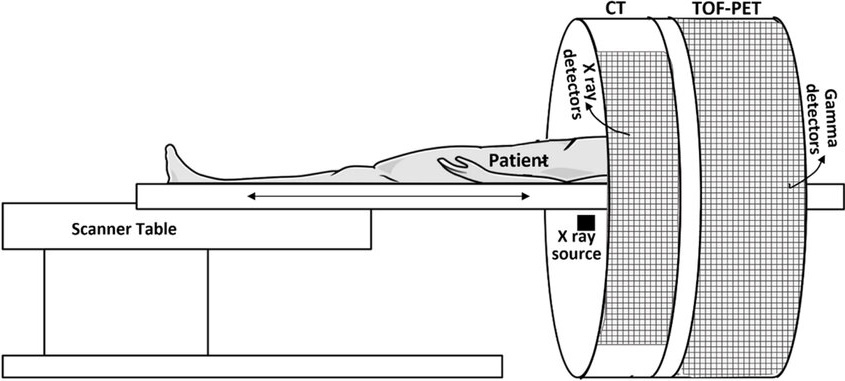
\includegraphics[width=0.45\textwidth]{assets/PETCTtable.jpg} 
	\caption{Schematic representation of TOF-capable PET/CT scanner with operational depiction of individual. Adapeted from Mohammadi \cite{figPETCT}}
	\label{fig:PETCTtable} 
\end{figure}

The device can be operatared separately or together within a single framework. In combined mode, CT images are employed for attenuation correction of PET data. When PET is used alone, it usually requieres for separate transmission scans used to provide anatomical reference and attenuation correction for images. Having them together improves imaging quaily while reducing examination time from additional scans \cite{townsend2004}%, zaidi2005}.

Clinical studies have demonstrated that even with shorter acquisition times, such as 1.5 minutes per bed position, image quality remains clinically acceptable with high rates of lesion visualization. PET/CT is a viable option for radiation workflows that are time-sensitive due to its efficiency and quality balance \cite{hasegawa2012}.


Modern PET/CT systems use advanced image registration techniques to improve data alignment and reduce errors.
Techniques for Deformable Image Registration (DIR), including GPU-accelerated DIR, take into consideration non-rigid changes brought on by patient movements or breathing patterns. 

Deformable Image Registration (DIR) methods such as, GPU-accelerated DIR, account for non-rigid transformations caused by patient motion or breathing patterns. These techniques model respiratory motion, improving the quantification and localization of functional uptake in PET imaging. In liver cancer treatment, where organ mobility presents major obstacles, such developments are very helpful \cite{shi2023}.

Additionally, this technique is considered upon its ability to detect non-FDG uptake lesions, contrasting with PET and helping avoid misdiagnosis in complex cases such as liver tumors \cite{yan2024, decazes2021}. This is done with segmentation algorithms that establish SUV thresholds to delineate lesions, integrating these volumes into treatment plans. Then, combining PET/CT with multiphasic CT can further characterize non-FDG lesions by leveraging dynamic contrast patterns visible in CT \cite{TG174}.

%\subsubsection{Dosimetry}
%PET/CT is generally used for dosimetry calcuations, an example of this will be found on liver cancer treatments such as Yttrium-90 (\(^{90}\text{Y}\)) in the appendix \ref{sec:case1}. 
Accurate dosimetry is dependent on quantitative imaging metrics such as standardized uptake values (SUVs). One of the advantages as explained in AAPMs TG174 and other papers is attenuation correction and faster acquisition times.\cite{knesaurek2018,TG174}. 

This system comes pre-integrated and aligns PET and CT datasets in the same frame of reference via software from the manufacturers and allows to acquire images in a single session ensuring precise alignment between functional and anatomical data.This reduces registration errors, ensuring precise tumor localization and dose delivery. 

CT imaging contributes with the electron density information necessary for attenuation correction in PET imaging. Since CT operates at lower photon energies (typically 80–140 keV), its data must be converted to match the 511 keV photons detected by PET. This calibration creates attenuation maps that align with PET imaging physics and are applied during PET image reconstruction to adjust the signal intensity, producing PET images that accurately represent metabolic activity without distortion due to tissue absorption.\cite{knesaurek2018, TG174}

In addition to attenuation correction, PET/CT facilitates tumor segmentation based on metabolic activity by converting PET data into standardized uptake values (SUVs). This information can then be integrated into radiotherapy planning systems to optimize treatment

Even with this seamless integration of the devices, respiratory motion and artifacts, particularly in liver cancer cases, can affect the accuracy of dose distribution. In TG174 we can find some techniques to mitigate respiratory motion artifacts in liver imaging as well as quality assurance (QA) protocols \cite{TG174}.

For example, TG174 highlights the use of respiratory gating to reduce motion artifacts caused by the liver’s movement during the breathing cycle. Or in the absence of respiratory gating, a time-weighted average intensity projection can mitigate the blurring effects of motion in PET intensity values.

Aside from this montly uniformity, quantification, and alignment tests between PET and CT datasets and annual Testing with phantoms, such as the ACR flangeless PET phantom, assesses PET/CT alignment and SUV accuracy are recomended.

Moreover, PET/CT tends to show lower SUV values compared to PET/MR, which may lead to underestimation of lesion uptake \cite{Prado-Wohlwend2023}. This underestimate can result in missed lesions, underestimation of disease severity, and incorrect staging of tumors. These limitations are particularly significant for liver imaging, where PET/MR has demonstrated increased diagnostic accuracy, with a 14.6\% improvement compared to PET/CT\cite{Prado-Wohlwend2023}.

In a case study, Knesaurek et al. \cite{knesaurek2018} reported differences in liver volume estimation between PET/CT and PET/MR, with a significant impact on dosimetry calculations. %The discussion on this finding can be found on section \ref{sec:case}.
 This means that by choosing the correct imaging system for planing can make a huge difference. 


\subsection{PET/MR}
On the flip side, a relatively new imaging modality has been catching some interest, and could provide complementary benefits to PET/CT in radiotherapy. PET/Magnetic Resonance Imaging (PET/MR), while not as established as PET/CT can still provide soft-tissue contrast and functional imaging capabilities that are quite attractive for specific liver cancer cases.

This integration allows the recording of functional and anatomical information concurrently. The three prime strategies for combining PET/MR imaging include the following that are sequential, insert an integrated systems. In the systems that are sequential, there arrangement whereby a patient is allowed to be scanned first in pet scanner and subsequently in an MR-type scanner; this is easily enabled by having a prepared mechanical bed for moving the patient. This modality combination is easy but does not allow  simultaneous imaging. Misalignment and space are certainly an issue. In insert systems, a PET detector ring is inserted into the bore of an existing MR scanner. This approach allows simultaneous acquisition, superior spatial, and temporal alignment; however, several technical problems, such as magnetic field interference and limited bore size, make it suitable for rather specific applications, like neurological studies \cite{ziegler2013}.


\begin{figure}[H]
	\centering
	% Subfigure a: Sequential
	\begin{subfigure}[b]{0.45\textwidth}
		\centering
		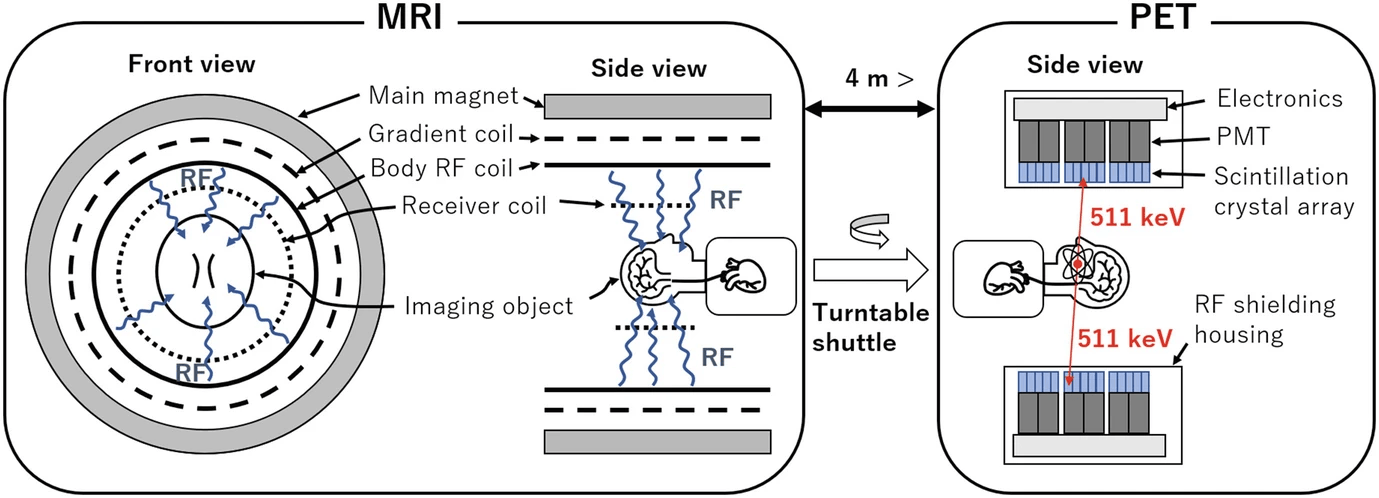
\includegraphics[width=\textwidth]{assets/sequencial.png}
		\caption{Sequential whole-body PET/MRI design using table shuttle for patient transportation.}
		\label{fig:sequential}
	\end{subfigure}
	% Subfigure b: Insert
	\begin{subfigure}[b]{0.45\textwidth}
		\centering
		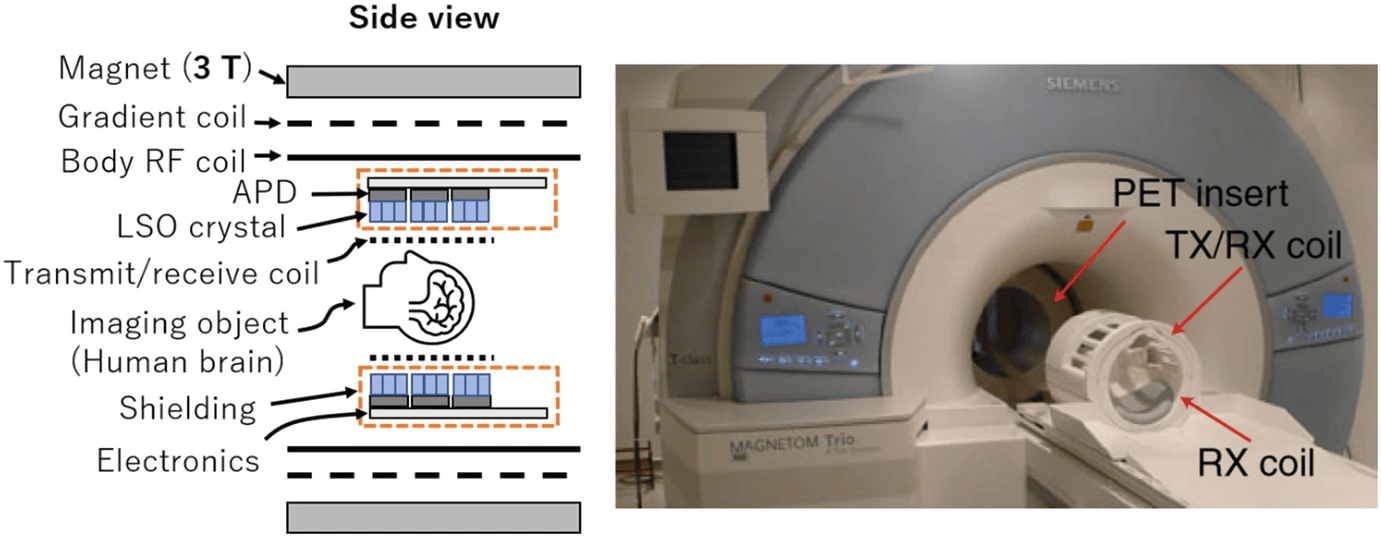
\includegraphics[width=\textwidth]{assets/insert.png}
		\caption{Schematic diagram of the APD-based brain PET insert with 3 T MRI and a photo of the brain PET insert combined with a slightly modified clinical 3 T MRI (right).}
		\label{fig:insert}
	\end{subfigure}
	
	% Subfigure c: Integrated
	\begin{subfigure}[b]{0.45\textwidth}
		\centering
		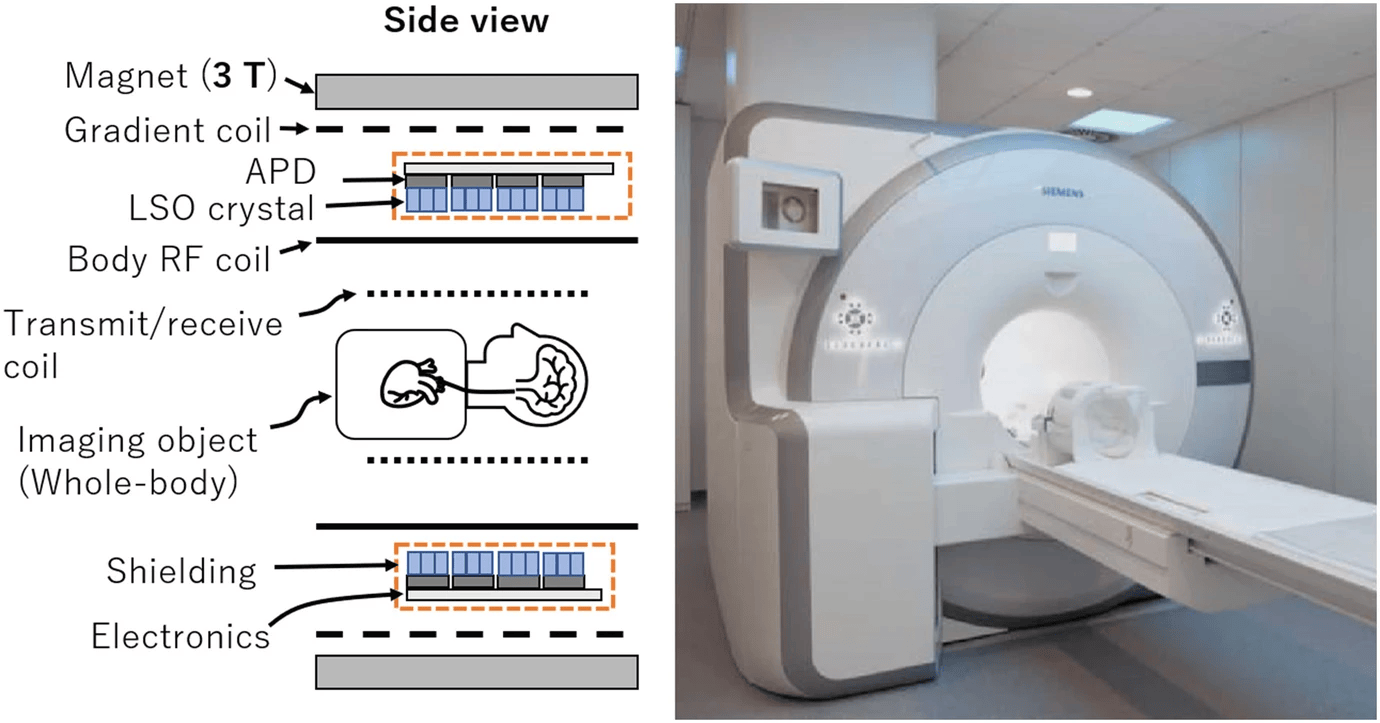
\includegraphics[width=\textwidth]{assets/integrated.png}
		\caption{Schematic diagram (left) and photo (right) of the first commercially available fully integrated whole-body PET/MR with APD technology.}
		\label{fig:integrated}
	\end{subfigure}
	
	\caption{Comparison of different PET/MRI configurations: (a) Sequential system, (b)Insert-based brain PET system. , and (c) Fully integrated system. Adapted from \cite{Kang2021}.}
	\label{fig:pet_mri_configurations}
\end{figure}

Integrated PET/MR systems are defined as the direct integration of the PET detectors inside the MR scanner. Most common embodiments place the PET detector ring behind the radiofrequency coil of the MR scanner using a split superconducting magnet or field-cycled MR in order to be able to house the PET components. PET detectors in PET/MR systems are prepared by using materials that will not perturb the magnetic field and degrade the quality of MR images. Situating the detectors at the rear of the radiofrequency coil increases temperatures and may cause their oscillations. This is important because the gain of both APDs and SiPMs-commonly used in the construction of PET systems-depend on temperature \cite{ziegler2013}%,Muzic2014}. Schematics on each of these implamentations of the system are shown in figure \ref{fig:pet_mri_configurations}.


%\subsubsection{Soft Tissue Contrast}
Having better soft tissue contrast in the abdominal area aids the planning process by accurately delineating liver tumors from healthy tissue. Instead of relying on CT attenuation correction, MR benefits the patient with reduced radiation dose and better delineation of anatomical structures \cite{knesaurek2018}. This is really valuable for cases with small or poorly defined tumors.

Additionally, PET/MR’s ability to image respiratory liver motion during PET acquisition provides more reliable data for motion management compared to PET/CT \cite{knesaurek2018}. High-resolution MR images can also assist in partial volume corrections for PET images, further enhancing the precision of tumor targeting, but lacks electron density making attenuation correction challeging.

%\subsubsection{Functional Imaging}
PET by itself comes with functional data from the activity distribution, but MR will enhance this capabilities if combined with techniques like DWI (Diffusion-Weighted Imaging) and dynamic contrast-enhanced (DCE) imaging, for additional parameters on tumor metabolism and treatment response. 

\textbf{Diffusion-Weighted Imaging (DWI):} This technique assesses the movement of water molecules within tissues by measuring the Apparent Diffusion Coefficient (ADC). Tumors often exhibit lower ADC values due to high cellularity and restricted diffusion caused by cell membranes. Treatment-related changes in ADC values can reflect alterations in cellularity, serving as an early marker of therapeutic response \cite{pmc2010}%, ajr2006}.

\textbf{Dynamic Contrast-Enhanced (DCE) MRI:} DCE MRI tracks the distribution of contrast agents over time, providing valuable insights into blood flow and vascular integrity. Changes in perfusion patterns frequently correlate with treatment response, as increased perfusion often indicates effective therapy \cite{academic2021}.

Effective treatments typically lead to increased ADC values, reflecting reduced cellularity as tumor cells die. These changes can be observed within days to weeks after chemotherapy or radiotherapy. However, early treatment may cause transient decreases in ADC due to cellular swelling or vascular changes, necessitating careful interpretation \cite{pmc2010}%, pmc2009}.
Combining DCE MRI with PET data creates a multiparametric approach, integrating metabolic activity from PET with blood flow characteristics from DCE MRI. This synergy enhances the understanding of tumor behavior and supports personalized therapeutic strategies \cite{springer2024}%,frontiers2020}.

MR is already a solid tool for advance planning as explained in TG284\cite{TG284}. Despite these advantages, the longer acquisition times and lack of specific guidelines for PET/MR integration by AAPM make this technique rise questions. However, its use may be justified in cases where soft-tissue contrast is critical for treatment success. 

PET/MR contribute in a unique way to the planing and staging part, the following sections are to explore how this is implemented with radiation therapy and what is the overall effect on target delineation and dosimetry.



\subsection{PET/MR usage on Radiation Therapy}

%Yans Fig. 1 | Comparison of PET/MRI for radiotherapy procedures with conventional radiotherapy procedures
Figure \ref{fig:petmri_vs_conventional} shows the simplified workflow made possible by PET/MRI, compared to conventional radiotherapy procedures. According to Yan et al. \cite{yan2024}, PET/MRI greatly improves efficiency, eliminates the need for multiple devices, and minimizes mistakes from co-registration processes by integrating imaging and positioning steps into a single operation.

\end{multicols}

\begin{figure}[H]
\centering
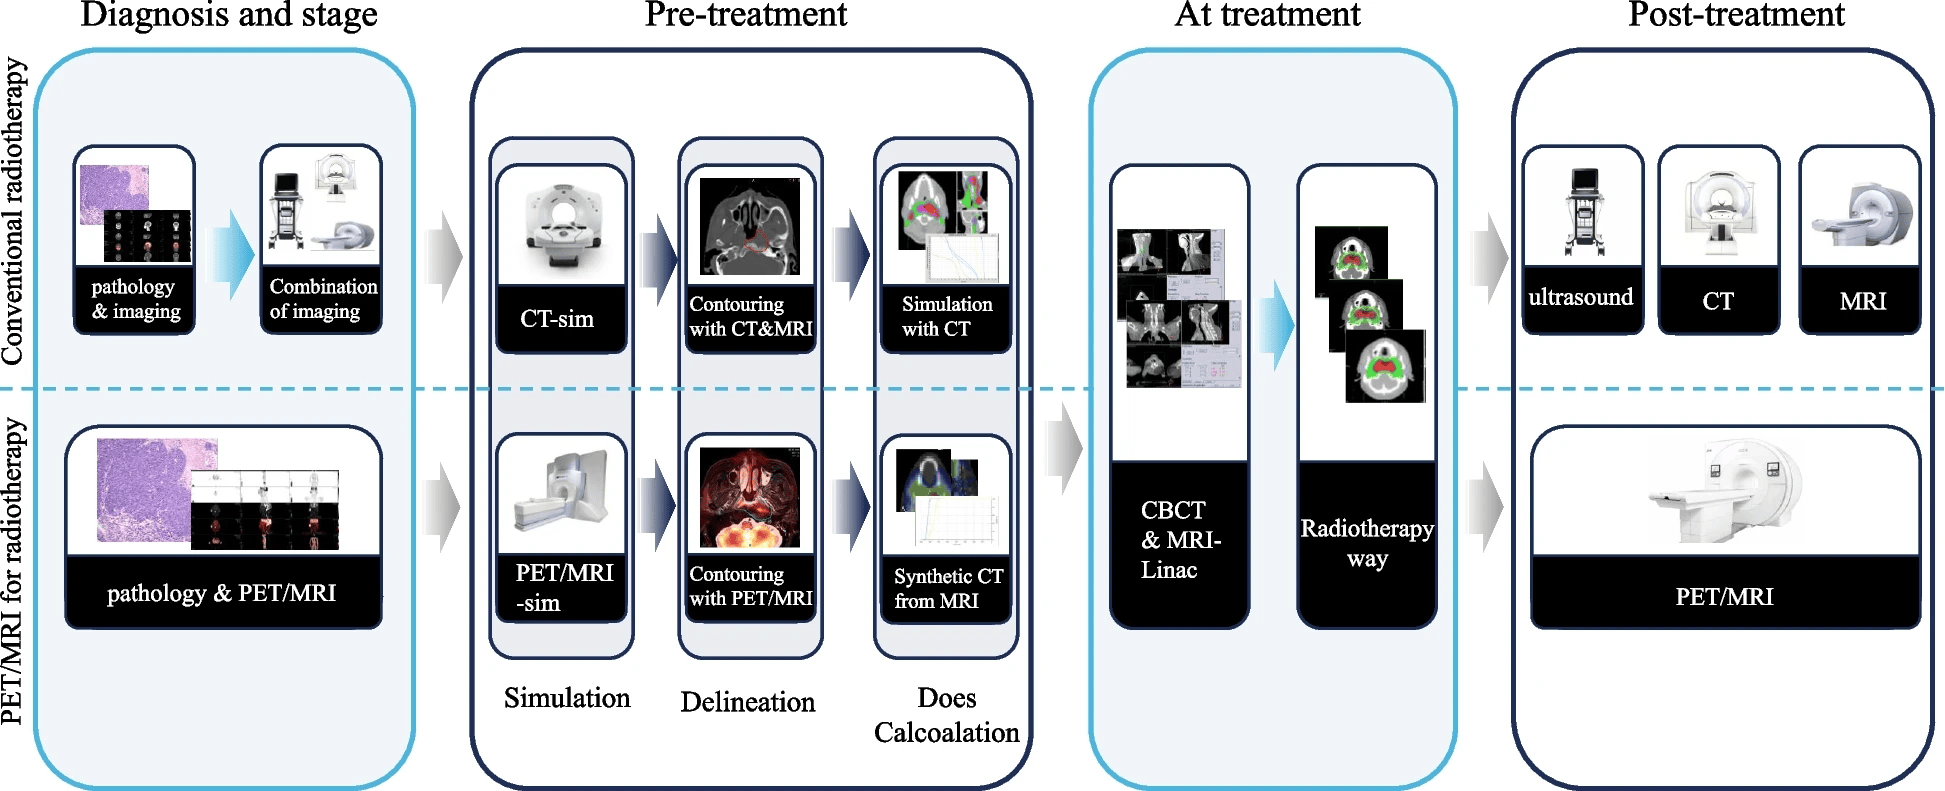
\includegraphics[width=1\textwidth]{assets/PETMRI_vs_Conventional_Workflow.png}
\caption{Comparison of PET/MRI workflows for radiotherapy procedures with conventional radiotherapy procedures. Adapted from Yan et al. \cite{yan2024}.}
\label{fig:petmri_vs_conventional}
\end{figure}


\begin{multicols}{2}

According to Decazes et al., adopting PET/MRI into radiation procedures needs careful planning and adjustments, that include using synthetic CT (pseudo-CT) for volume delineation and attenuation correction. %how would this be done
By immobilizing the patient, PET/MR allows for alignment between imaging modalities without the need for further registration procedures. In order to provide precise dosimetry planning without the need for several imaging devices, artificial intelligence methods, such GANs, further optimize attenuation mapping and shorten the pre-treatment routine \cite{decazes2021}.

%needs further explanation and development

\subsection{Positioning, Planning, and Pretreatment Workflow}

\paragraph{Specific Equipment and Material}
In order to properly use PET/MR in the clinical setting, challenges regarding patient positioning need to be addressed due to PET/MR's  unique design and functional requirements compared to PET/CT. The following discussion is primarily informed by Yan et al. \cite{yan2024}.
Regarding equipment, a regular curved diagnostic MR couch is unsuitable for PET. Instead, the use of flat treatment couch allows consistent patient positioning across imaging and treatment sessions while minimizing photon attenuation. Photon attenuation is further addressed in the materials used. Conventional carbon fiber tables, while minimally attenuating photons, can create surface currents that degrade MR image quality. Hybrid materials, such as plastic-foam sandwiches, have been developed to reduce photon attenuation and eliminate artifacts. Additionally, thin plastic shells and lightweight coil technologies are being explored to optimize attenuation correction (AC) without compromising image quality. \cite{yan2024, ziegler2013}

\paragraph{Effect on Image Quality}
The integration of these devices and materials influences the signal-to-noise ratio (SNR) and overall image quality. Phantom studies have shown negligible effects on SNR between flat and curved tables. However, positioning devices increase the distance between the patient and MR coils, reducing SNR by approximately 25\%. This reduction does not significantly impact target delineation accuracy. Techniques such as increasing the signal average, lowering acceleration factors, such as the reduction of parallel imaging acceleration, can also enhance SNR, or modifying echo times (e.g., by optimizing the echo spacing for a given tissue type) can improve image contrast and mitigate SNR loss, though these adjustments may increase acquisition time. \cite{yan2024,Rostami2024}

\paragraph{Attenuation Correction}
Due to the lack of CT in these devices, attenuation correction is a major challenge. For example, rigid hardware such as coil holders and flat tables are usually accounted for using CT-based 3D AC maps or isotope-based attenuation maps; this is no longer the case for PET/MR. There is a need to introduce coil fixation devices that mitigate errors caused by the variable positioning of flexible RF coils during scanning to improve reliability of AC maps. Moreover, there is a bone segmentation limitation. MR-based AC often excludes bone due to the low intensity of bone signals in MR images. Atlas-based methods, which use pre-existing templates of CT anatomy to generate a pseudo-CT for attenuation correction, can incorporate bone structures but may introduce registration errors in regions with varying stiffness, such as the abdomen.

Overall, consistent positioning is critical to ensure reliable imaging and proper AC. Studies using phantoms have demonstrated minimal deviations in accuracy during multiple repositioning with RF coil holders. Additionally, PET/MR simulator tables allow single registration for fixed tabletop setups, ensuring repeatability in radiation therapy workflows.

\paragraph{Target delineation}
Tumor delineation in radiotherapy involves the definition of at least 3 different volumes, gross tumor volume (GTV), clinical target volume (CTV), and planning target volume (PTV). PET/MR offers unique advantages over conventional imaging modalities, particularly in refining GTV boundaries by integrating both morphological and biological data.


MRI alone is commonly used to outline the GTV based on tumor morphology, while PET provides additional biological insights that mitigate the risk of marginal misses. Studies cited in Yan et al. demonstrate Zhang et al.’s \cite{Zhang2014} observation that PET imaging contributed to an approximate 10\% increase in tumor volume detection not captured by MRI alone.\cite{yan2024} This finding better explains tumor sizes measured under a microscope, it is also supported by comparisons of Dice Similarity Coefficient (DSC), a metric used to assess the overlap between imaging-based tumor delineations and the ground truth, he explains.%who? i think Zhang

This difference on the outline of the GTV is shown in figure \ref{fig:gtv_delineation_cropped}, while it focuses on nasopharyngeal cancer, it provides valuable insights into the comparative performance of PET/MRI and PET/CT for tumor delineation. Soft-tissue contrast of PET/MRI is especially relevant for complex tumor regions, such as the liver.

%Yans Fig. 3 | Nasopharyngeal GTV delineations across modalities

%	•	Highly relevant to tumor delineation discussions but less so for liver cancer.
%	•	Acknowledge that it focuses on nasopharyngeal cancer while emphasizing generalizable findings.


\begin{figure}[H]
	\centering
	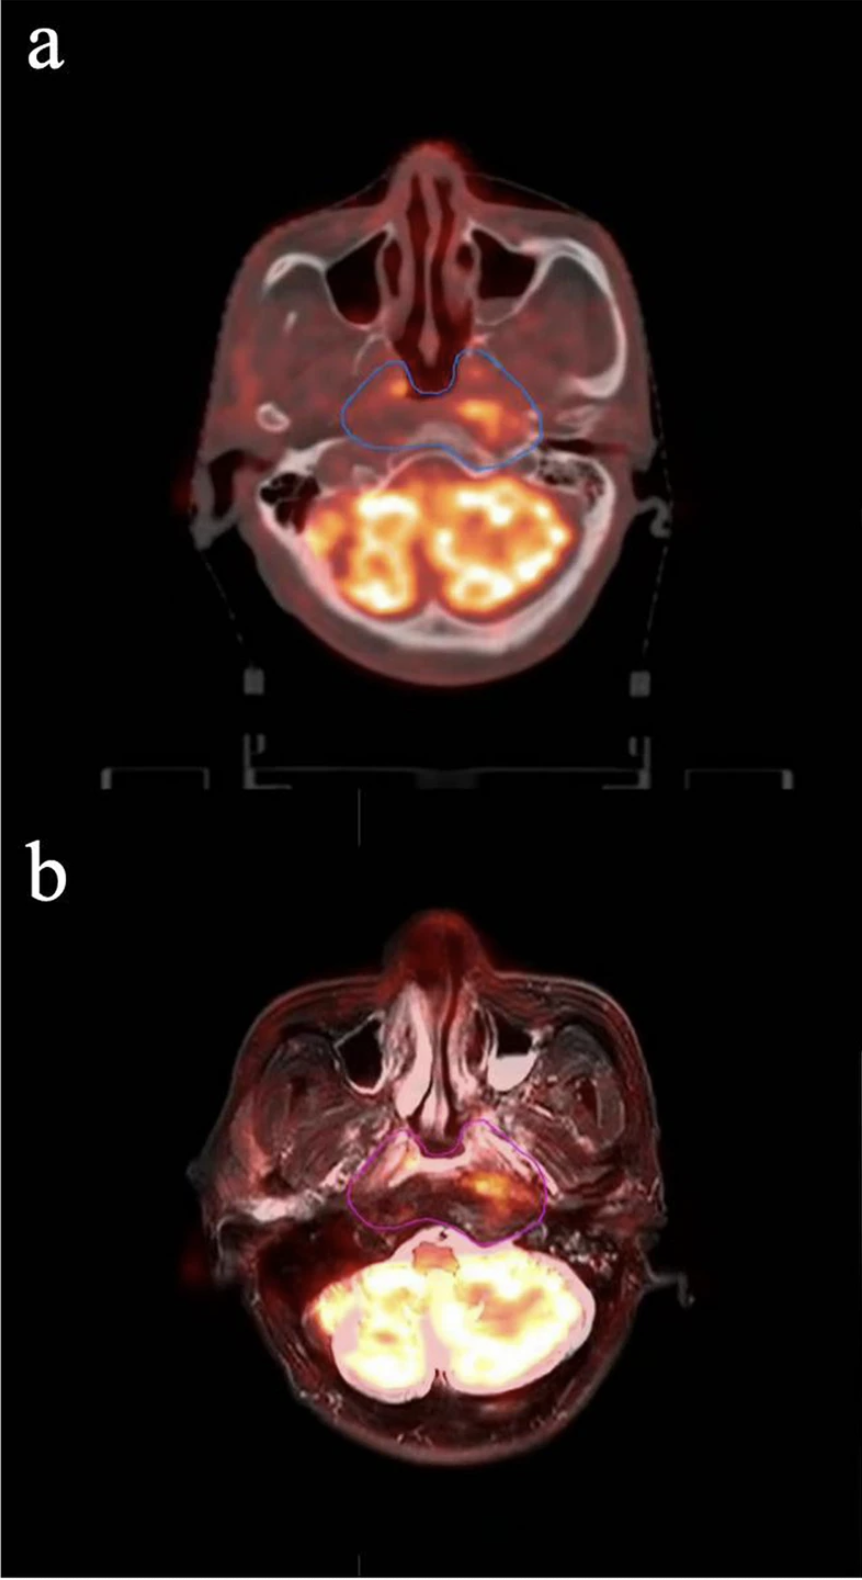
\includegraphics[width=0.8\columnwidth]{assets/GTV_Delineation_PETCT_vs_PETMRI.png} 
	\caption{Gross tumor volume (GTV) delineation across PET/CT and PET/MRI modalities for a 69-year-old female with nasopharynx cancer. (a) The blue line represents GTV-PET/CT. (b) The pink line represents GTV-PET/MRI. Adapted from Yan et al. \cite{yan2024}.}
	\label{fig:gtv_delineation_cropped}
\end{figure}

The addition of PET provides some advantages as well, PET’s ability to capture tumor biology introduces the concept of Biological Target Volume (BTV), which integrates metabolic and functional characteristics of tumors. Using BTV data, radiotherapy can deliver higher doses to treatment-resistant regions while sparing sensitive areas. This approach, known as "dose painting" or "dose sculpting," aims to increase cure rates without increasing late radiation-induced toxicity. \cite{Schinagl2006}

Of course there are limitations, starting from manual tumor delineation, though widely used, it introduces significant variability. To address this, adaptive thresholding based on individual standardized uptake values (SUVmax) and automated delineation methods are being explored. For example, PET/MRI’s co-segmentation methods have been shown to match observer performance in target delineation while providing more consistent results across repeated evaluations \cite{yan2024}. And regarding its comparison to PET/CT, PET/MR has reduced SUVmax values that may lead to conservative tumor boundaries.

The integration of PET in radiotherapy planning has led to significant alterations in radiation treatment volumes for 30\%-60\% of non-small cell lung cancer (NSCLC) patients. \cite{Bradley2004}. PET/CT has improved stereotactic body radiation therapy (SBRT) treatment in NSCLC patients by advancing the development of prognostic PET/CT radiomic signatures \cite{Vijayakumar2022}.

\paragraph{Dose Calculation and Optimization}

Once the target volume is delineated, the next step of planing is dose calculations. For PET/MR there are technical considerations compared to PET/CT, particularly in the context of SBRT, where precision in dose distribution is everything.

The main challenge presented on PET/MR is that it lacks the capability to directly acquire tissue electron density values. As of right now workflows include co-register PET/MR with CT images to generate dose prescription maps. Studies found that pseudo-CT techniques generated from MR images have high accuracy, and reported negligible mean absolute errors of 0.17 ± 0.12 Gy in dosimetry analysis \cite{yan2024}.

However, PET/MR offers significant advantages for SBRT planning, particularly in reducing radiation exposure. Time-of-Flight (TOF) PET/MR systems require only 35\% of the activity concentration needed for TOF-PET/CT while maintaining comparable image quality, translating to a theoretical dose reduction of up to 65\%, with clinical observations suggesting realistic reductions exceeding 50\% \cite{Polan2023}%,Queiroz2015}. 

\subsubsection{Mid-Treatment Workflow}

In accordance with Yan et al., [18F]-FDG PET/MRI mid-treatment assessments offer essential details on tumor response using metrics that include $\Delta \text{SUVmax}$ and $\Delta \text{Dmin}$. Their function is to provide predictions for treatment sensitivity and risk of recurrence. Significant changes in water transport and glucose metabolism were noted throughout treatment, allowing for adaptive therapy modification to prevent toxicity or accelerated tumor development \cite{yan2024}.  

A way to take advantage from this preparation, incorporating PET-based absorbed dose map into mid-treatment workflows for SBRT or SIRT is possible. Polan et al. (2023) studied how sequentially integrating $^{90}\text{Y}$-PET-based dose distribution clinicians were able to refine treatment plans, enhancing the precision of dose delivery and adapting to dynamic tumor changes during therapy \cite{Polan2023}. 

Addditionally, studies have shown that  advanced techniques, such as Intensity-Modulated Radiation Therapy (IMRT) and Volumetric Modulated Arc Therapy (VMAT), particularly benefit from advanced imaging techniques by leverage real-time anatomical and functional imaging to adjust dose distributions dynamically \cite{Hunte2022}%,Tsang2016}.

Referencing back to Figure \ref{fig:petmri_vs_conventional}, after using PET/MR and synthetic CT to performe treatment planing and dosimetric calculations, Cone-Beam Computed Tomography (CBCT) and MRI-guided Linear Accelerators (MRI-LINAC) are suggested for mid treatment assesment. CBCT provides high-resolution imaging of anatomical structures, enabling precise verification of patient positioning and tumor morphology before and during treatment. By capturing volumetric data, CBCT facilitates precise target localization and minimizes setup uncertainties, a key requirement for the high precision demanded in SBRT \cite{Srinivasan2014}.

MRI-LINAC, on the other hand, combines the superior soft-tissue contrast of MRI with real-time radiation delivery. This integration allows clinicians to continuously monitor tumors and surrounding tissues with unparalleled clarity, enabling dynamic adjustments during treatment. They also are methodologies for adaptative therapy workflows. For SBRT, sub-millimeter precision is critical,  and MRI-LINAC ensures that the radiation dose is confined to the target while sparing adjacent organs at risk. The ability to visualize and adapt to changes in tumor size, shape, and position during therapy enhances the precision and safety of treatments. Furthermore, MRI-LINAC supports adaptive planning workflows, as demonstrated by Lei et al. (2020) and Cunningham et al. (2022), where the incorporation of synthetic MRI and cine MRI imaging techniques have significantly improved tumor tracking and dose conformity in SBRT \cite{Lei2020}%,Cunningham2022}.
\end{multicols}

\begin{multicols}{2}

%\FloatBarrier % Prevents floats from going past this point

\section{Discussion}
% ============================
% Section: Discussion
% ============================


%\subsection{Improved Targeting Accuracy}
Better tumor delineation can be archived with the use of hybrid imaging modalities. They provide unique features like the integration of anatomical and biological data that allows for improvements. More precise treatment planning is possible as this approach advances; this is especially true for body parts with intricate tumor borders or areas that move a lot, like the liver.

By capturing metabolic and vascular behavior, the combination of functional imaging modalities including Diffusion-Weighted Imaging (DWI) and Dynamic Contrast-Enhanced (DCE) imaging allows for improved tumor characterisation in PET/MR.

%\subsection{Implications for Liver Cancer Management}
By considering the potential of new and linked technologies on liver cancer management will transform therapeutic approaches, soft tissue contrast and functional imaging of PET/MR is really promising. cases with small, poorly defined and unresectable tumors will be benefited from these advantages and developments. As PET/MR becomes more widely adopted, its role in adaptive radiotherapy workflows and personalized treatment regimens could improve survival rates and quality of life for liver cancer patients.

The idea of biological target volumes (BTV) is also introduced by the incorporation of PET/MR into radiation operations, opening the door to sophisticated techniques like dose painting. This approach allows higher doses to be delivered to treatment-resistant regions while sparing healthy tissue, ultimately improving therapeutic outcomes. Additionally, pseudo-CT creation in PET/MR can simplify processes, cutting down on treatment planning time and complexity.


%In Appendix \ref{sec:case}, a case study on $^{90}\text{Y}$ microsphere treatment is shown to further demonstrate the usefulness of PET/CT and PET/MR imaging in radiation planning. This case highlights key differences in dosimetry, motion management, and imaging parameters between PET/CT and PET/MR, underscoring their respective advantages in radiotherapy workflows.

\section{Limitations and Future Directions}
% ============================
% Section: Limitations and Future Directions
% ============================


%\subsection{Challenges of PET/MR Integration}

Despite its advantages, PET/MR has logistical and technical difficulties. The most obvious ones are the extended acquisition times and higher costs. Second to that, consider the limited availability in clinical settings and integration with current techniques. Furthermore, the lack of standardized attenuation correction methods and sensitivity to motion artifacts is a huge deterrent. Addressing these issues will require advancements in imaging technology, standarized protocols and better workflow integration.\cite{pichler2008,Prakken2023}

%\subsection{Need for AAPM Guidelines}
To fully realize the potential of PET/MR in radiotherapy, comprehensive guidelines from professional organizations like AAPM are necessary. These guidelines (like they do for PET/CT) should address dosimetry protocols, motion management techniques, and the development of pseudo-CT methods for attenuation correction or alternatives. Further research is needed to establish the clinical efficacy of PET/MR in routine practice and optimize its role in radiotherapy workflows.


\section{Conclusion}
% ============================
% Section: Conclusion
% ============================
This paper compares the advantages and limitations of PET/CT and PET/MR in liver cancer radiotherapy, it has a focus on their impact on tumor delineation, dosimetry, and treatment planning. PET/CT remains the gold standard for many clinical applications and PET/MR demonstrates significant potential in improving targeting accuracy and providing superior soft-tissue contrast and additional functional imaging capabilities, such as Diffusion-Weighted Imaging (DWI) and Dynamic Contrast-Enhanced (DCE) imaging.

Dose painting and other adaptive radiotherapy methods are made possible by the special potential for improved tumor characterisation that come with PET/MR integration. These advances are particularly relevant for complex cases involving small, poorly defined, or unresectable liver tumors. Despite these advantages, obstacles including longer acquisition times, more expenses, and the lack of standardized attenuation correction techniques prevent PET/MR from being widely used.


Future research and the development of standardized protocols will set the way in overcoming current limitations and ensuring these technologies achieve their full clinical potential in precision radiotherapy.

\end{multicols}

\newpage
% ============================
% Appendix
% ============================

\begin{appendices}
	
\begin{multicols}{2}	
	\section{Supplementary Case Applications: }
	% ============================
% Section: Case Application - 90Y Microsphere Therapy
% ============================

\label{sec:case}

To illustrate the usefulness and problems of PET/MR a case application is presented. The comparison of PET/CT and PET/MRI for post-therapy quantitative imaging of Yttrium-90 (90Y) distribution given by Knesaurek et al. \cite{knesaurek2018} is followed.

Yttrium-90 (90Y) microsphere therapy, also known as Selective Internal Radiation Therapy (SIRT) %Underscored SIRT
, is an emerging treatment for unresectable hepatic tumors. This therapy delivers targeted radiation with microspheres loaded with 90Y with the objective of spare healthy tissues and concentrate the dose within tumors.

Although both techniques offer information on tumor dosimetry, their unique benefits and drawbacks must be carefully considered before being used in clinical settings. This section explores imaging parameters, dosimetry results, and tumor delineation findings, with a focus on their implications for radiotherapy planning and outcomes.

In Knesaurek et al.’s prospective study, 32 patients underwent sequential imaging on a PET/CT system and a PET/MR system immediately following 90Y-SIRT. The PET/CT acquisition used a Siemens Biograph mCT system with time-of-flight (TOF) capabilities and low-dose CT scans were employed for attenuation correction. PET/MR imaging was performed using a Siemens Biograph mMR system, which uses avalanche photodiodes (APDs) instead of photomultiplier tubes but lacks TOF capabilities. 
Attenuation correction for PET/MR relied on four-tissue segmentation derived from Dixon sequences, %Needs explanation how?
to compensate for the lack of CT-based corrections. Imaging parameters included matrix size, voxel sizes and acquisition times. 

%wrote: Not SBRT...

Both modalities implemented advanced reconstruction algorithms: Poisson-ordered subset expectation maximization (OP-OSEM3D) with TOF and point spread function (PSF) for PET/CT, and OP-OSEM3D with PSF for PET/MR. Validation was conducted through a phantom study using a 90Y-filled Jaszczak sphere, that ensured cross-calibration and consistency in dosimetry across the systems.

%Knešaureks Fig. 1 | Phantom study comparing PET/CT and PET/MRI for 90Y calibration
% visually support system calibration.

Figure \ref{fig:phantom_petct_petmri} demonstrates the results of that phantom study, it compares PET/CT and PET/MRI systems for $^{90}\text{Y}$ calibration. Results indicate that both systems are closely calibrated for \(^{90}\text{Y}\) with less than 1\% difference.

\begin{figure*}[ht]
	\centering
	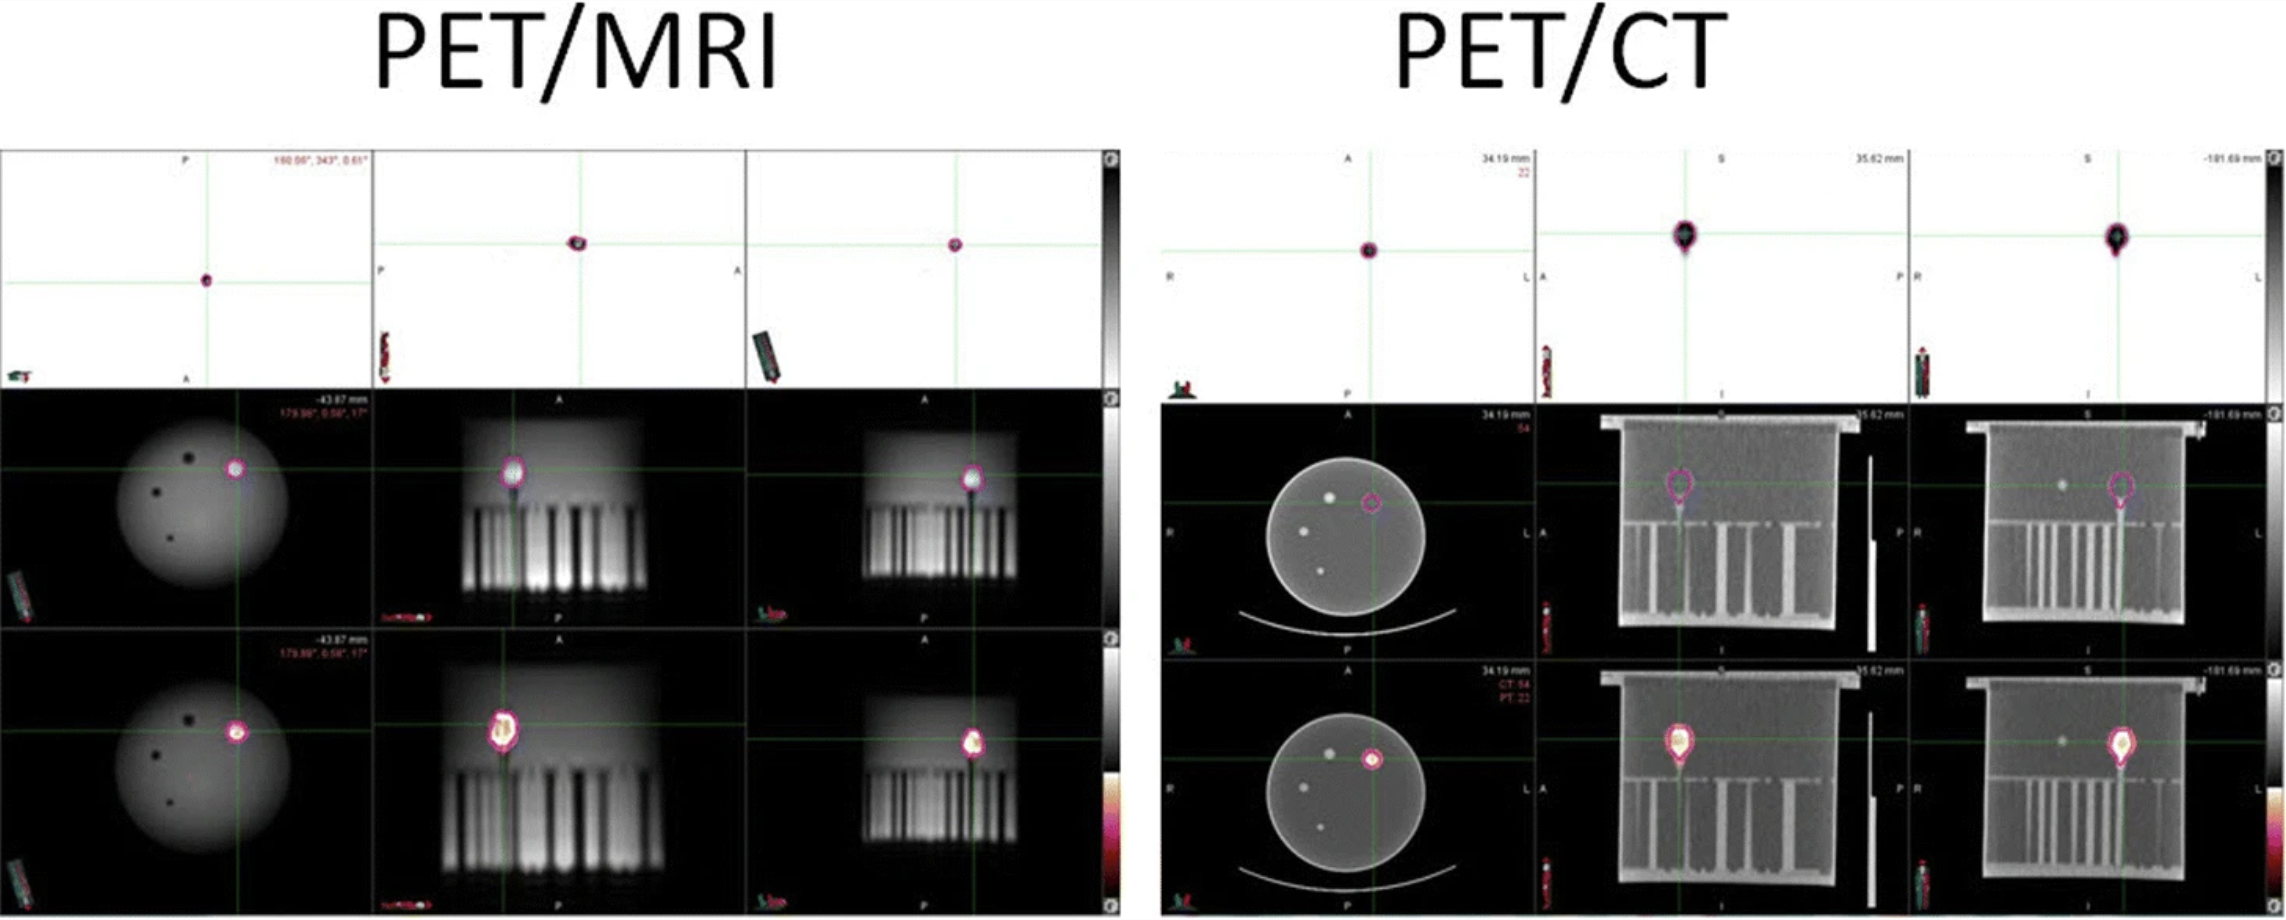
\includegraphics[width=0.9\textwidth]{assets/PETCT_vs_PETMRI_Phantom.png} % Replace with the correct file path
	\caption{Phantom study comparing PET/CT and PET/MRI for \(^{90}\text{Y}\) calibration. The top row displays PET images, the middle row shows MRI and CT images respectively, and the bottom row presents fused PET/MRI and PET/CT images.  Adapted from Knešaurek et al. \cite{knesaurek2018}.}
	\label{fig:phantom_petct_petmri}
\end{figure*}

This methodology provides a foundation for analyzing tumor delineation, motion management, soft-tissue contrast, and dosimetric accuracy between PET/CT and PET/MR. The following sections discuss these aspects.

\subsubsection{Target delineation}

\paragraph{Image Registration and Fusion.} 

PET/CT simultaneous acquisition ensure spatial consistency across datasets \cite{TG132}. This simplifies radiotherapy planing, particularly in workflows that require direct integration into treatment planning systems. 

PET/MR relies on deformable image registration to align PET data with MR images, as the datasets are acquired using different mechanisms and frames of reference. % needs explanation

The challenge here are the errors produced by differences on the anatomy contrast and the distortions from MRI technique.

Knesaurek et al. \cite{knesaurek2018}, exemplifies this with the need to implement and use a vast collection of MRI sequences for delineation and creation of tumor ROIs. 

%revise
\paragraph{Motion Management}

There are different approaches to address motion artifacts during the acquisition of the images, for liver cancer is significant because of its location near the diaphragm. PET/CT relies on gated acquisition or time-weighted averaging methods to account for motion blur, but these methods are limited in capturing the full range of liver motion \cite{Dhont2020}. 

PET/MR offers an advantage as it can see motion during PET with MR motion correction sequences %wrote ? underscored MR motion correction sequences
aiding in reconstruction and reducing artifacts\cite{knesaurek2018}. Dhont et al. \cite{Dhont2020} noted that motion-resolved PET/MR provides better tumor localization and volume estimation for motion-prone tumors, potentially improving dose escalation accuracy.

Applying motion correction techniques, %How is this done?
such as those available in PET/MRI systems, could mitigate these effects and improve reliability in T/N ratio calculations \cite{knesaurek2018}. This is particularly important in cases where respiratory motion introduces artifacts, as shown in Figure \ref{fig:respiratory_motion_artifacts}, which demonstrates $^{90}\text{Y}$ spillover into the lungs during PET/CT imaging due to diaphragm motion.

%Knešaureks Fig. 4 | Respiratory motion artifacts and spillover with 90Y
%	Relevant if discussing motion artifacts

\begin{figure*}[ht]
	\centering
	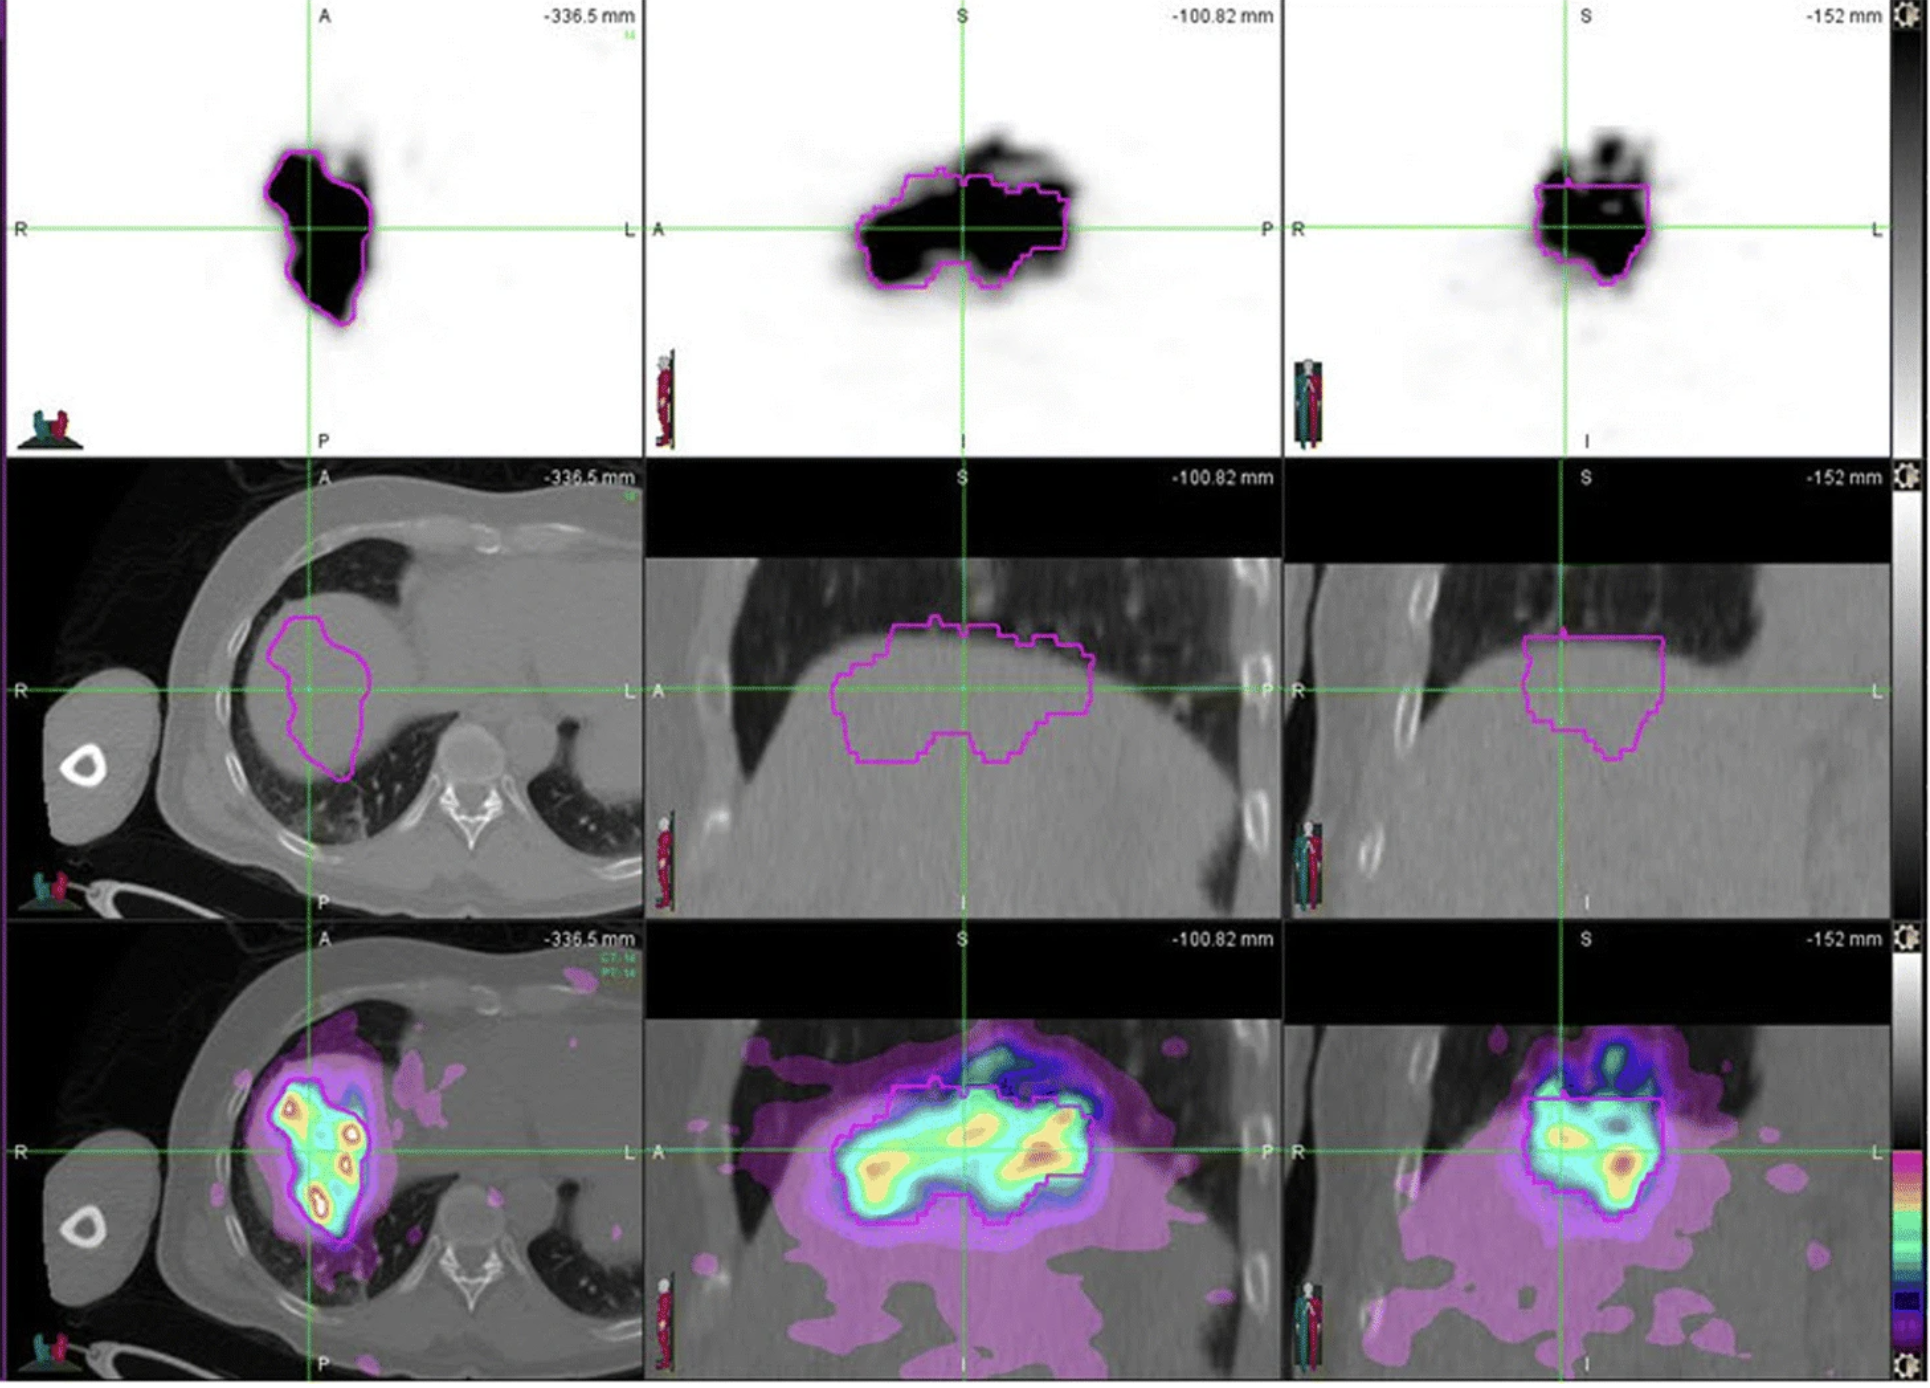
\includegraphics[width=0.9\textwidth]{assets/Respiratory_Motion_Artifacts.png} 
	\caption{Respiratory motion artifacts and spillover with \(^{90}\text{Y}\) imaging using PET/CT. The top row displays uncorrected PET images in axial (left), sagittal (middle), and coronal (right) views. The middle row shows the corresponding CT anatomical references, and the bottom row presents fused PET/CT images, where spillover into the lungs due to respiratory motion is evident. Adapted from Knešaurek et al. \cite{knesaurek2018}.}
	\label{fig:respiratory_motion_artifacts}
\end{figure*}



\paragraph{Soft-Tissue Contrast}

The most significant advantage of PET/MR lies in soft-tissue contrast, with proper contrast comes better differentiation of liver tumors from healthy tissue and surrounding structures:

PET/MR is particularly effective for delineation small liver tumors ($<$2 cm), where partial volume effects in PET/CT can compromise visualization. \cite{knesaurek2018} Also it is demonstrated that ROIs derived from MR images allow more precise tumor targeting in challenging cases, such as when tumors are indistinct in CT. %wrote Liver? SBRT?


\paragraph{Acquisition Time and Workflow}

The total acquisition time for PET/CT is largely determined by the PET component, as CT acquisition takes only seconds. This efficiency makes PET/CT the preferred choice for high-throughput settings\cite{knesaurek2018}.
While in PET/MR, acquisition time is dictated by the MR component, which can significantly increase scan duration due to the need for multiple MR sequences. %why?
While this trade-off is justified for cases requiring detailed anatomical or functional imaging, it limits PET/MR’s utility in busy clinical workflows \cite{knesaurek2018}.

%wrote in general for this page moslty surface description without significant development on physics or clinical
%lots of material & opportunities to explain the physics / tecnical / approach in detail

\subsubsection{Dosimetry}
At the end a solid argument to be made in favor of an imaging technique for treatment planning revolves around dosimetry. Dosimetry impacts treatment efficacy and seeks to minimize damage to healthy tissue. The main differences between PET/CT and PET/MR reside on their technical characteristics leading to distinct applications and limitations.

\paragraph{Attenuation Correction and Quantitative Accuracy.}

The fact that PET/CT are a single system is a huge advantage as CT provides attenuation correction. More reliable SUV values and dose calculations will result from the high-density resolution of CT all this while having a reproducible attenuation correction across a wide range of tissues

The MR attenuation correction is less accurate, the lack of direct bone density mapping may lead to underestimation of attenuation in osseous structures on the surrounding areas. Moreover, MR AC requires segmentation of tissues into predefined classes (e.g., air, soft tissue, fat, bone). Liver cancer imaging often deals with heterogeneous structures (e.g., cirrhotic livers, metastases). Errors in segmentation directly impact ROI creation and subsequent dosimetry calculations. 


Following the work of Knesaurek, \cite{knesaurek2018} PET/CT typically provides slightly higher SUVmean and SUVmax values compared to PET/MR, which may lead to discrepancies in tumor delineation and dosimetry calculations. The mean liver dose for $^{90}\text{Y}$ therapy was 51.6 Gy with PET/CT and 46.5 Gy with PET/MR, with differences attributed to variations in attenuation correction and liver volume estimation.

%figure 4 is way down may shift once following sections are done
Figure \ref{fig:patient_liver_dose} shows the liver dosimetry differences between PET/CT and PET/MRI in a patient study. It is important to notice the variations in attenuation correction and liver volume estimation. The mean liver dose obtained from PET/CT was 38.81 Gy, while PET/MRI measured 31.64 Gy, with differences attributed to variations in attenuation correction and liver volume estimation.

%Knešaureks Fig. 2 | Patient study with highest mean liver dose difference
%highlight liver dosimetry differences.
\begin{figure*}[ht]
	\centering
	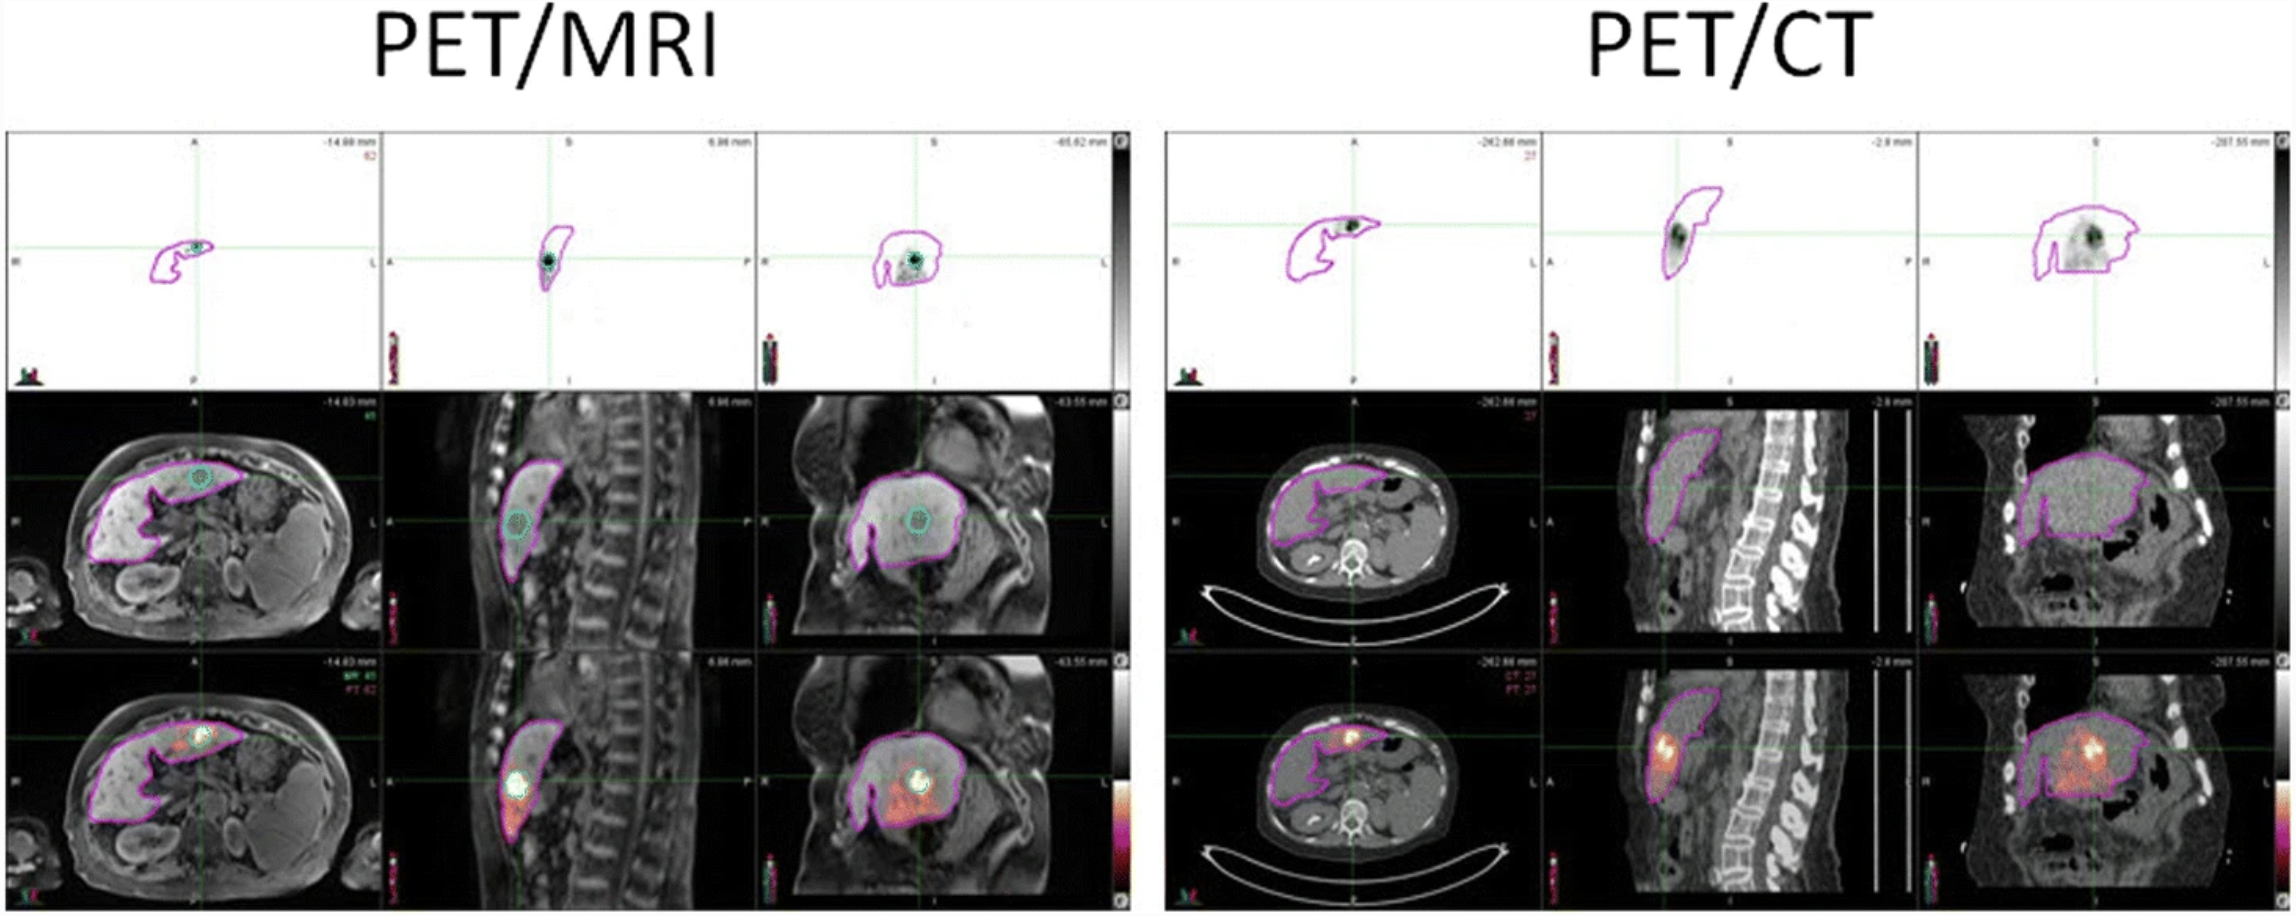
\includegraphics[width=0.9\textwidth]{assets/Liver_Dosimetry_Differences.png} 
	\caption{Patient study showing the highest mean liver dose difference between PET/CT and PET/MRI. The top row displays PET images, the middle row shows MRI and CT images respectively, and the bottom row presents fused PET/MRI and PET/CT images. Adapted from Knešaurek et al. \cite{knesaurek2018}.}
	\label{fig:patient_liver_dose}
\end{figure*}

\paragraph{Partial Volume Effects}

Both PET/CT and PET/MR suffer from the imaging limitation of Partial volume effects (PVE). It occurs due to signal averaging across tissue borders inside a voxel. Then, tasks like tumor segmentation become more difficult as a result of the blurring edges and decreased precision in defining volumes of interest. 

PET/CT has a broad field of view and good tumor-to-node contrast, but its poorer spatial resolution and vulnerability to PVE make it difficult to quantify since they can cloud tumor borders. Fortunately PET/MRI can be utilized to correct PVE in PET pictures because of MRI's higher soft-tissue contrast and great spatial resolution. 

Knesaurek et al. \cite{knesaurek2018} reported that partial volume effects (PVEs) significantly impact quantification and dosimetry calculations, particularly for small tumors. Both modalities analyzed a tumor volume of approximately 7.0 $\text{cm}^3$ and mentions no use of contrast media. Intra hepatic dosimetry calculations of T/N ratios, requires using of contrast in anatomical modalities, as well as,
PV corrections for lesions smaller than 2.5 $\text{cm}$. And respiratory motion contributes the challenge of accurate T/N ratio estimation for undersized lesions, also noticible in figure \ref{fig:respiratory_motion_artifacts}.

\paragraph{Tumor-to-Normal Tissue Ratios (T/N Ratios)}

Thanks to soft-tissue contrast, which aids in more precise tumor delineation, PET/MR will have a higher T/N ratio. In organs like the liver this should be a requirement in order to spare and distinguish tumors from healthy liver tissue or adjacent structures.


On the other hand, PET/CT has the benefit of more precise attenuation correction, allowing for more accurate dose estimations and standardized uptake value (SUV) calculations. However, its accuracy in detecting tiny tumor boundaries gets limited by its poorer soft-tissue contrast as compared to PET/MR, especially when no contrast medium is present. This displays the way PET/MR can be preferable when dealing with complicated anatomy, such as the liver, by offering better distinction.


Knesaurek et al. \cite{knesaurek2018} managed to calculate T/N ratios for the PET/CT scan by leveraging MRI-derived tumor ROIs merged with CT images through deformable transformation, a process that aligns images from different modalities to a common coordinate system, in MIM software. The study reported T/N ratios of 24.90 for PET/CT and 30.00 for PET/MRI. 

Additionally, the absence of contrast agents in both CT and MRI images likely reduced the accuracy of tumor delineation and intra-hepatic dosimetry. The findings highlight the potential of PET/MRI to achieve superior T/N ratios (delivering higher relative doses to tumor regions), but also emphasize the importance of integrating advanced techniques like PVE corrections, contrast agents, and motion management into dosimetric workflows for small liver tumors.


	% =====================================
% Section:Examples on Imaging modalities on SBRT
% =====================================

\label{sec:case2}


In the this section an exploration of common use of PET/CT for SBRT on the liver as well as the use of MRI its reviewed. The intention of this section is to ground the previous findings with some clincal examples.

\section*{Integrating respiratory-gated PET-based target volume delineation in liver SBRT planning}

In an previous study on assesment of PET/CT for liver stereotactic body radiation therapy (SBRT) planning. 8 patients with 14 metastases were imaged. They used CT for attenuation correction and six PET phases were reconstructed. They aimed to compare images for target delination purposes incorporating respiratory gating technics. \cite{Riou2014}

They were able to find one undiagnosed metastasis in the respiratory gated part and allowed for a better defition on the PTV. In figure \ref{fig:liver-metastasis-PET} we can see some of their results. The first image shows the CT scan, then a PET scan and then combined, and shows CTV in dark blue, PTV in light blue, BITV in red and PTVg in magenta. 

\begin{figure}[H]
	\centering
	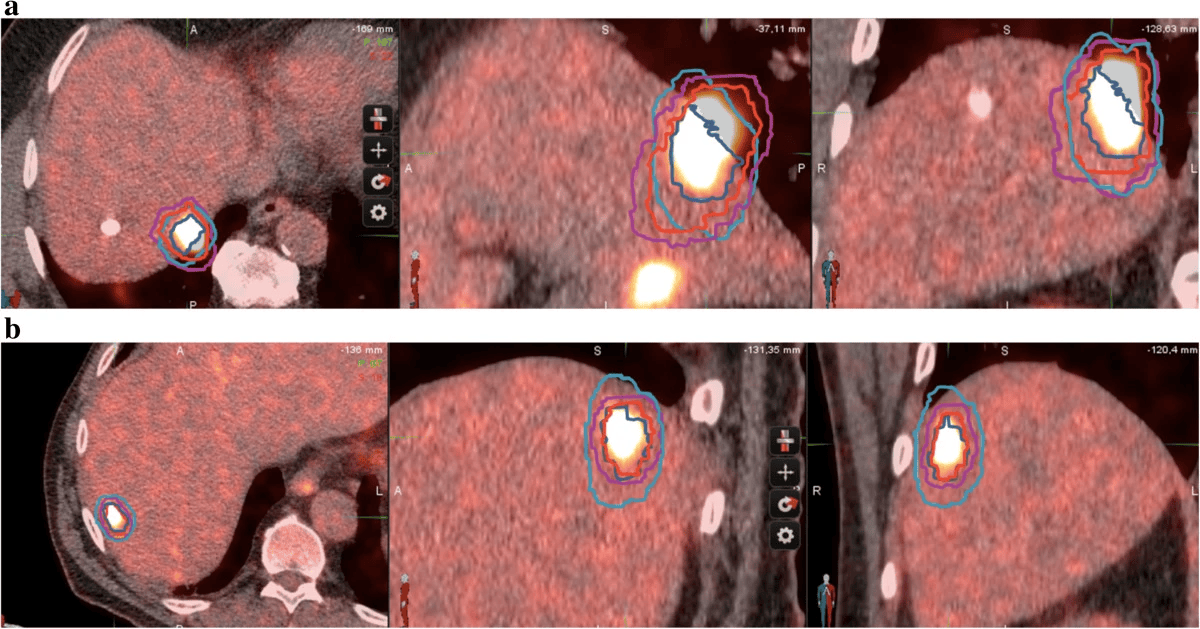
\includegraphics[width=0.5\textwidth]{assets/PETSBRTcomplete.png}
	\caption{Different target volumes obtained for a liver metastasis next to the diaphragm.\cite{Riou2014}}
	\label{fig:liver-metastasis-PET}
\end{figure}


\section*{Stereotactic MR-Guided Radiotherapy for Liver Metastases}

This study evaluates local treatment options for liver metastases, emphasizing the use of Stereotactic Body Radiation Therapy (SBRT). SBRT is a good choice for its ability to offer good local control and reduced toxicity levels, despite being a relatively novel application for liver conditions. Liver SBRT is a noninvasive technique that can be applied on an outpatient basis and is easy to combine sequentially with systemic treatments because of its excellent tolerance.

The study faced challenges previously established: liver metastases suffer from poor tissue contrast in X-ray imaging, complex anatomy requires advanced imaging, and breathing and diaphragm movement can prone to errors. The paper aims to solve this with the use of online cine MR sequences, MR Linac systems that combine gating (breath-hold treatments) and live tracking.

The authors reported a prospective registry covering treatments from October 2019 to April 2022. They treated 26 patients for 31 lesions using stereotactic MR-guided radiotherapy (MRgRT). According to their findings, nearly 90\% of the patients had been previously treated for one or more hepatic metastases, primarily through systemic treatment. Patient selection was conducted by a multidisciplinary tumor board and a technical board, assessing eligibility for MRgRT. The study included candidates with synchronous or metachronous oligo-metastatic liver metastases.

The researchers administered a radiation dose of 50 Gy in 5 fractions for 54.8\% of the lesions, with the dose increased to 60 Gy for 25\% of the lesions. They reported a median Planning Target Volume (PTV) of 35.6 cc, with a range from 9.9 to 343.2 cc. An adaptive protocol was implemented for 16.1\% of the lesions. Bordeau et al.\cite{bordeau2023}. The study protocol involved patients undergoing both contrast-enhanced CT and 0.35T MRI simulations using the MRIdian® system. These simulations, when registered with enhanced 1.5T MRI, improve the precision and effectiveness of the Stereotactic Body Radiation Therapy (SBRT) planning.


\begin{figure}[H]
	\centering
	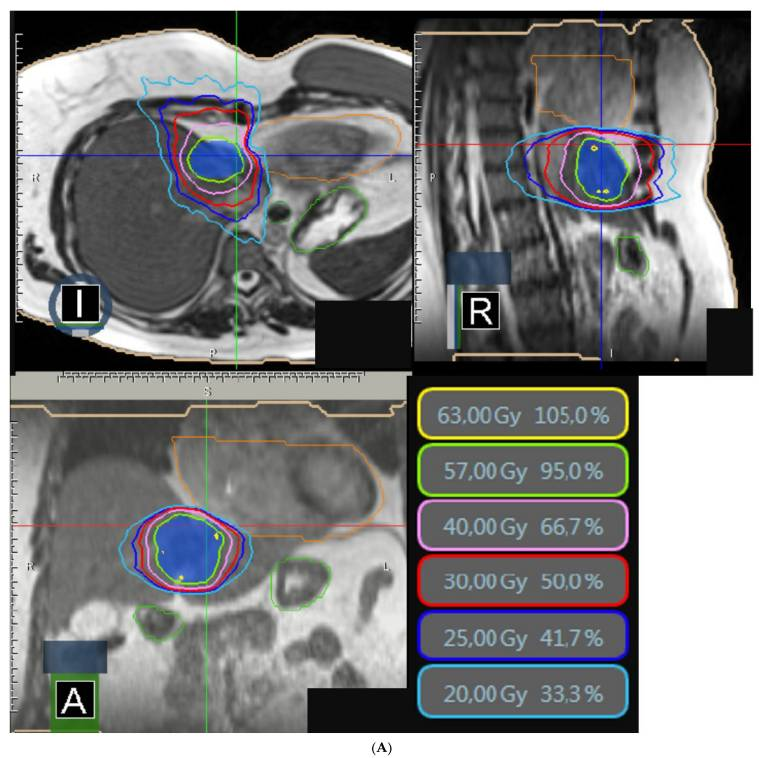
\includegraphics[width=0.5\textwidth]{assets/MRISBRT.jpeg}
	\caption{Dosimetry example for a liver metastasis from breast cancer. Planning Target Volume (PTV) shown in blue colorwash with isodose lines.\cite{bordeau2023}}
	\label{fig:liver-metastasis-dosimetry}
\end{figure}

In their results, they included no MRgRT-related acute toxicities. However they reported gastrointestinal toxicity, and late toxicities that were related to metastatic disease progression. They confirmed the feasibility and good tolerance of the treatment in that indication. Acute and late gastrointestinal and liver toxicities were low and mostly unrelated to MRgRT, they added. OAR were accounted for and monitored. 

\end{multicols}	

\end{appendices}


\bibliographystyle{unsrt} % Numbered references in order of appearance
\bibliography{references}

\end{document}